\section{Análise Experimental}

Por se tratar de um problema de otimização combinatória, rodamos cada experimento com 30 repetições. Todos os testes foram feitos em máquinas da Google através da plataforma Google Cloud. Os parâmetros variados nas execuções estão descritos na seção \ref{xp_par}. A análise experimental dos três \textit{datasets} estão divididas nas subseções seguintes.

O código pode ser executado pela linha de comando com os seguintes argumentos:

\begin{center}
\begin{verbatim}
    python3 main.py [-i ITERATIONS] [-a ANTS] [--alpha ALPHA] 
                    [--beta BETA] [--rho RHO] dataset
\end{verbatim}
\end{center}

\subsection{Parâmetros} \label{xp_par}

Os parâmetros são passados como argumentos na chamada do código. São eles:

\begin{itemize}
	\item Número de iterações(\textbf{Padrão}: 50) 
    \item Número de formigas((\textbf{Padrão}: $n - p$)
    \item Alpha(\textbf{Padrão}: 0.5) - Peso do feromônio do nó no cálculo da probabilidade.
    \item Beta(\textbf{Padrão}: 0.5) - Peso da heurística de informação no cálculo da probabilidade.
    \item Rho(\textbf{Padrão}: 0.9) - Taxa de evaporação do feromônio.
\end{itemize}

A semente mestra para o gerador aleatória é $123456$. A partir dela são geradas 30 outras sementes para serem usadas nas repetições. Ao fixarmos as sementes, permitimos que os resultados sejam reproduzíveis, caso necessário.

\subsection{Bases de dados}
3 bases de dados foram disponibilizadas para a realização dos experimentos: SJC1, SJC2 e SJC3b. Todas possuem números diferentes de nós, estes com características diferentes, e de medianas a serem encontradas. Os parâmetros foram variados um por um, sempre mantendo os valores padrões, como apresentados na subseção \ref{xp_par}, para aqueles que ficaram constantes naquela rodada de execuções.

\subsubsection{SJC1}

A base de dados SJC1 é composta de 100 pontos, todos com capacidade 720, mas com demanda variável. Ela busca por 10 pontos de mediana. Inicialmente buscamos entender o impacto do número de iterações no algoritmo. Como podemos ver na Figura \ref{fig:sjc1_iterations}, a medida que as iterações passam, melhor é a solução encontrada, como era de se esperar. 

\begin{figure}[h]	
  \centering
  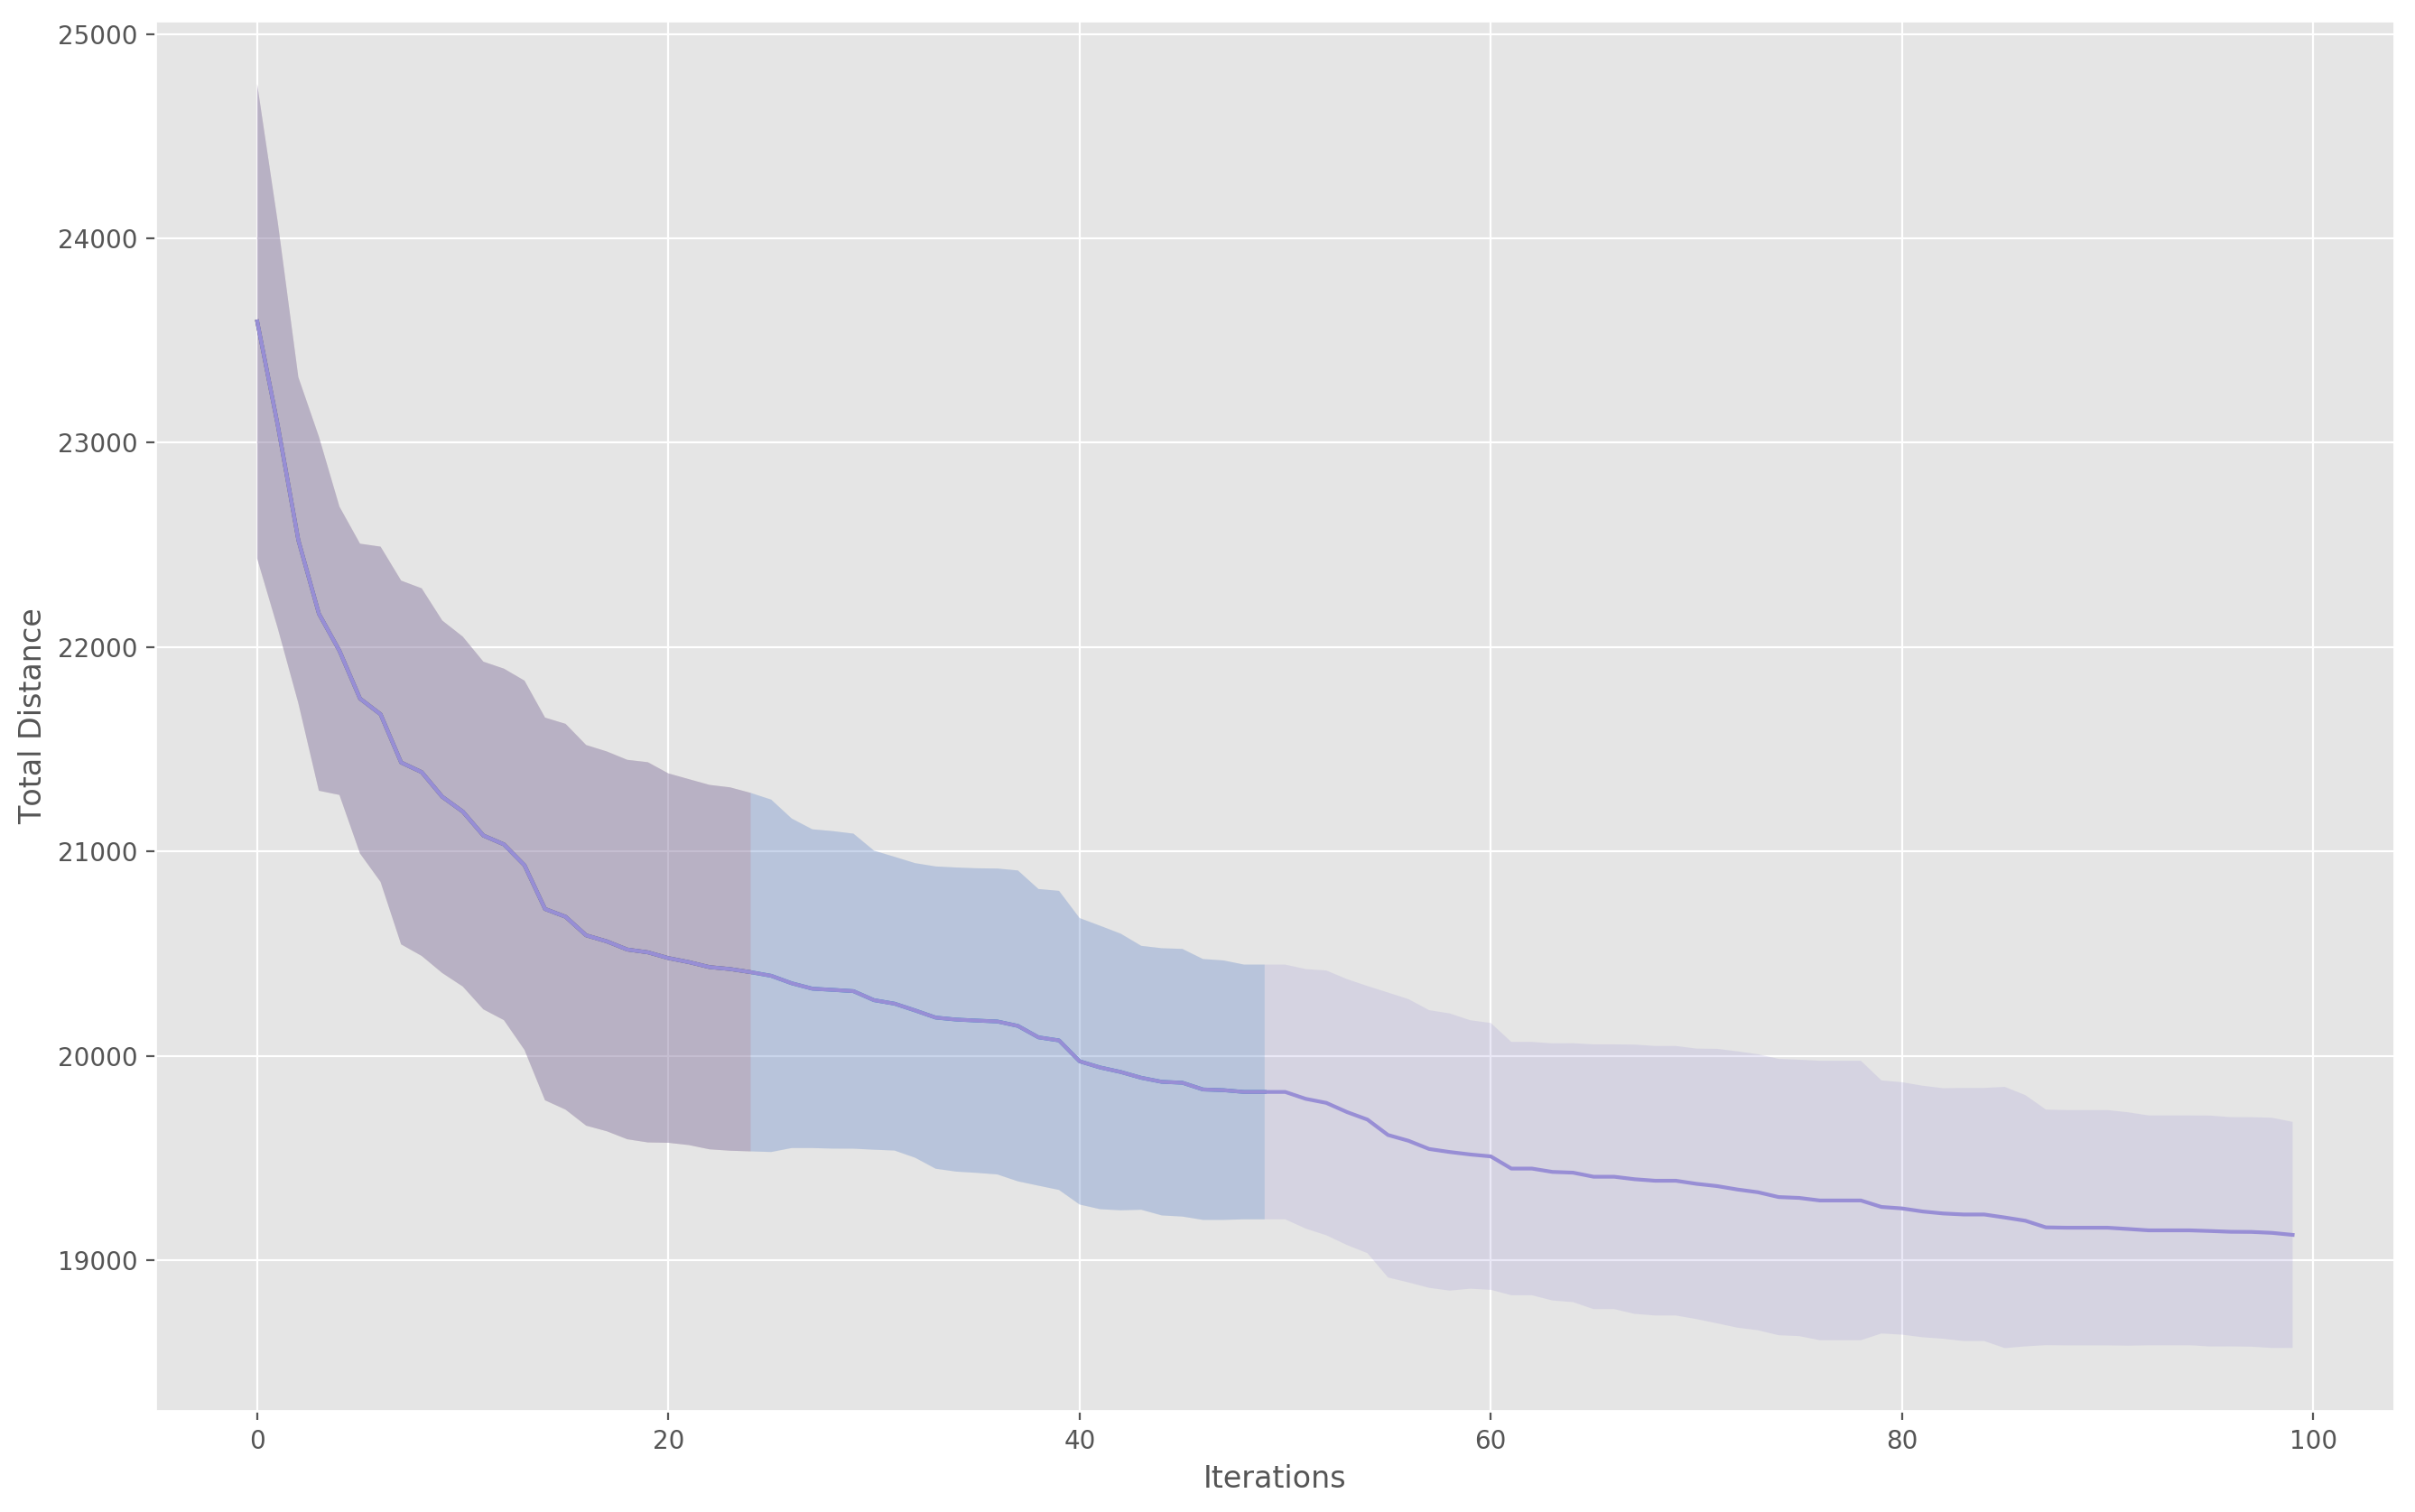
\includegraphics[width=11cm,keepaspectratio]{images/SJC1_iterations.png}
  \caption{Média e desvio padrão para a distância da solução encontrada para base SJC1 com número de iterações variável.}
  \label{fig:sjc1_iterations}
\end{figure}

Agora avaliaremos o que acontece quando variamos o número de formigas, e portanto o número de soluções geradas a cada iteração do algoritmo. Variamos as quantidade de formigas de acordo com $p$, $n - p$ e $2 * (n - p)$. A Figura \ref{fig:sjc1_ants}. Aqui algo inesperado acontece: após a iteração 32, e até a iteração final, tanto a média quanto o desvio padrão sofrem um mudança brusca. Isso aconteceu pois em uma das execuções, após essa iteração, a distância total cai de 21479 para 958. 

Analisando o porque esse foi o caso, chegou-se a conclusão de que o problema está provavelmente na detecção de estagnação presente no artigo. O fato aqui é que, aparentemente, o sistema converge antes do valor somado dos feromônios alcançar o total especificado na fórmula. Para tentar corrigir esse problema, um valor(0.5). para aumentar o \textit{range} de detecção de estagnação, adicionado à fórmula da seguinte forma:

\medskip
\begin{lstlisting}
if total_pheromone >= stagnation_threshold - 0.5:
	is_stagnated = True
\end{lstlisting}
\medskip
    
Esse valor foi encontrado empiricamente e resolveu para muitos casos, falhando raramente. O problema é que quando o sistema estagna, ele gera as mesmas soluções para todas as formigas, ou seja, o melhor e o pior valores locais são os mesmos e portanto a fórmula apresentada na subseção \ref{sub:update-pheromone} fica com um denominador igual a 0, fazendo com o que o algoritmo pare de funcionar corretamente.

Outra hipótese é a de que os valores padrão(0.5) de \textit{alpha} e \textit{beta}, que causam uma radiciação quando utilizados na fórmula da probabilidade, acabam gerando valores inválidos em raras ocasiões, causando o mesmo problema do denominador nulo. É estranho o fato de que nem \cite{de2005max} e nem o próprio criador do ACO, Marco Dorigo, em \cite{dorigo2003ant} citam essa provável ocorrência, o que me leva a acreditar na primeira hipótese.

Ao ignorarmos o resultado errado, encontramos o resultado que era de se esperar nesse teste: quanto mais formigas melhor. Portanto, $2 * (n - p)$ se mostrou o mais eficiente para encontrar soluções melhores.

\begin{figure}[h]	
  \centering
  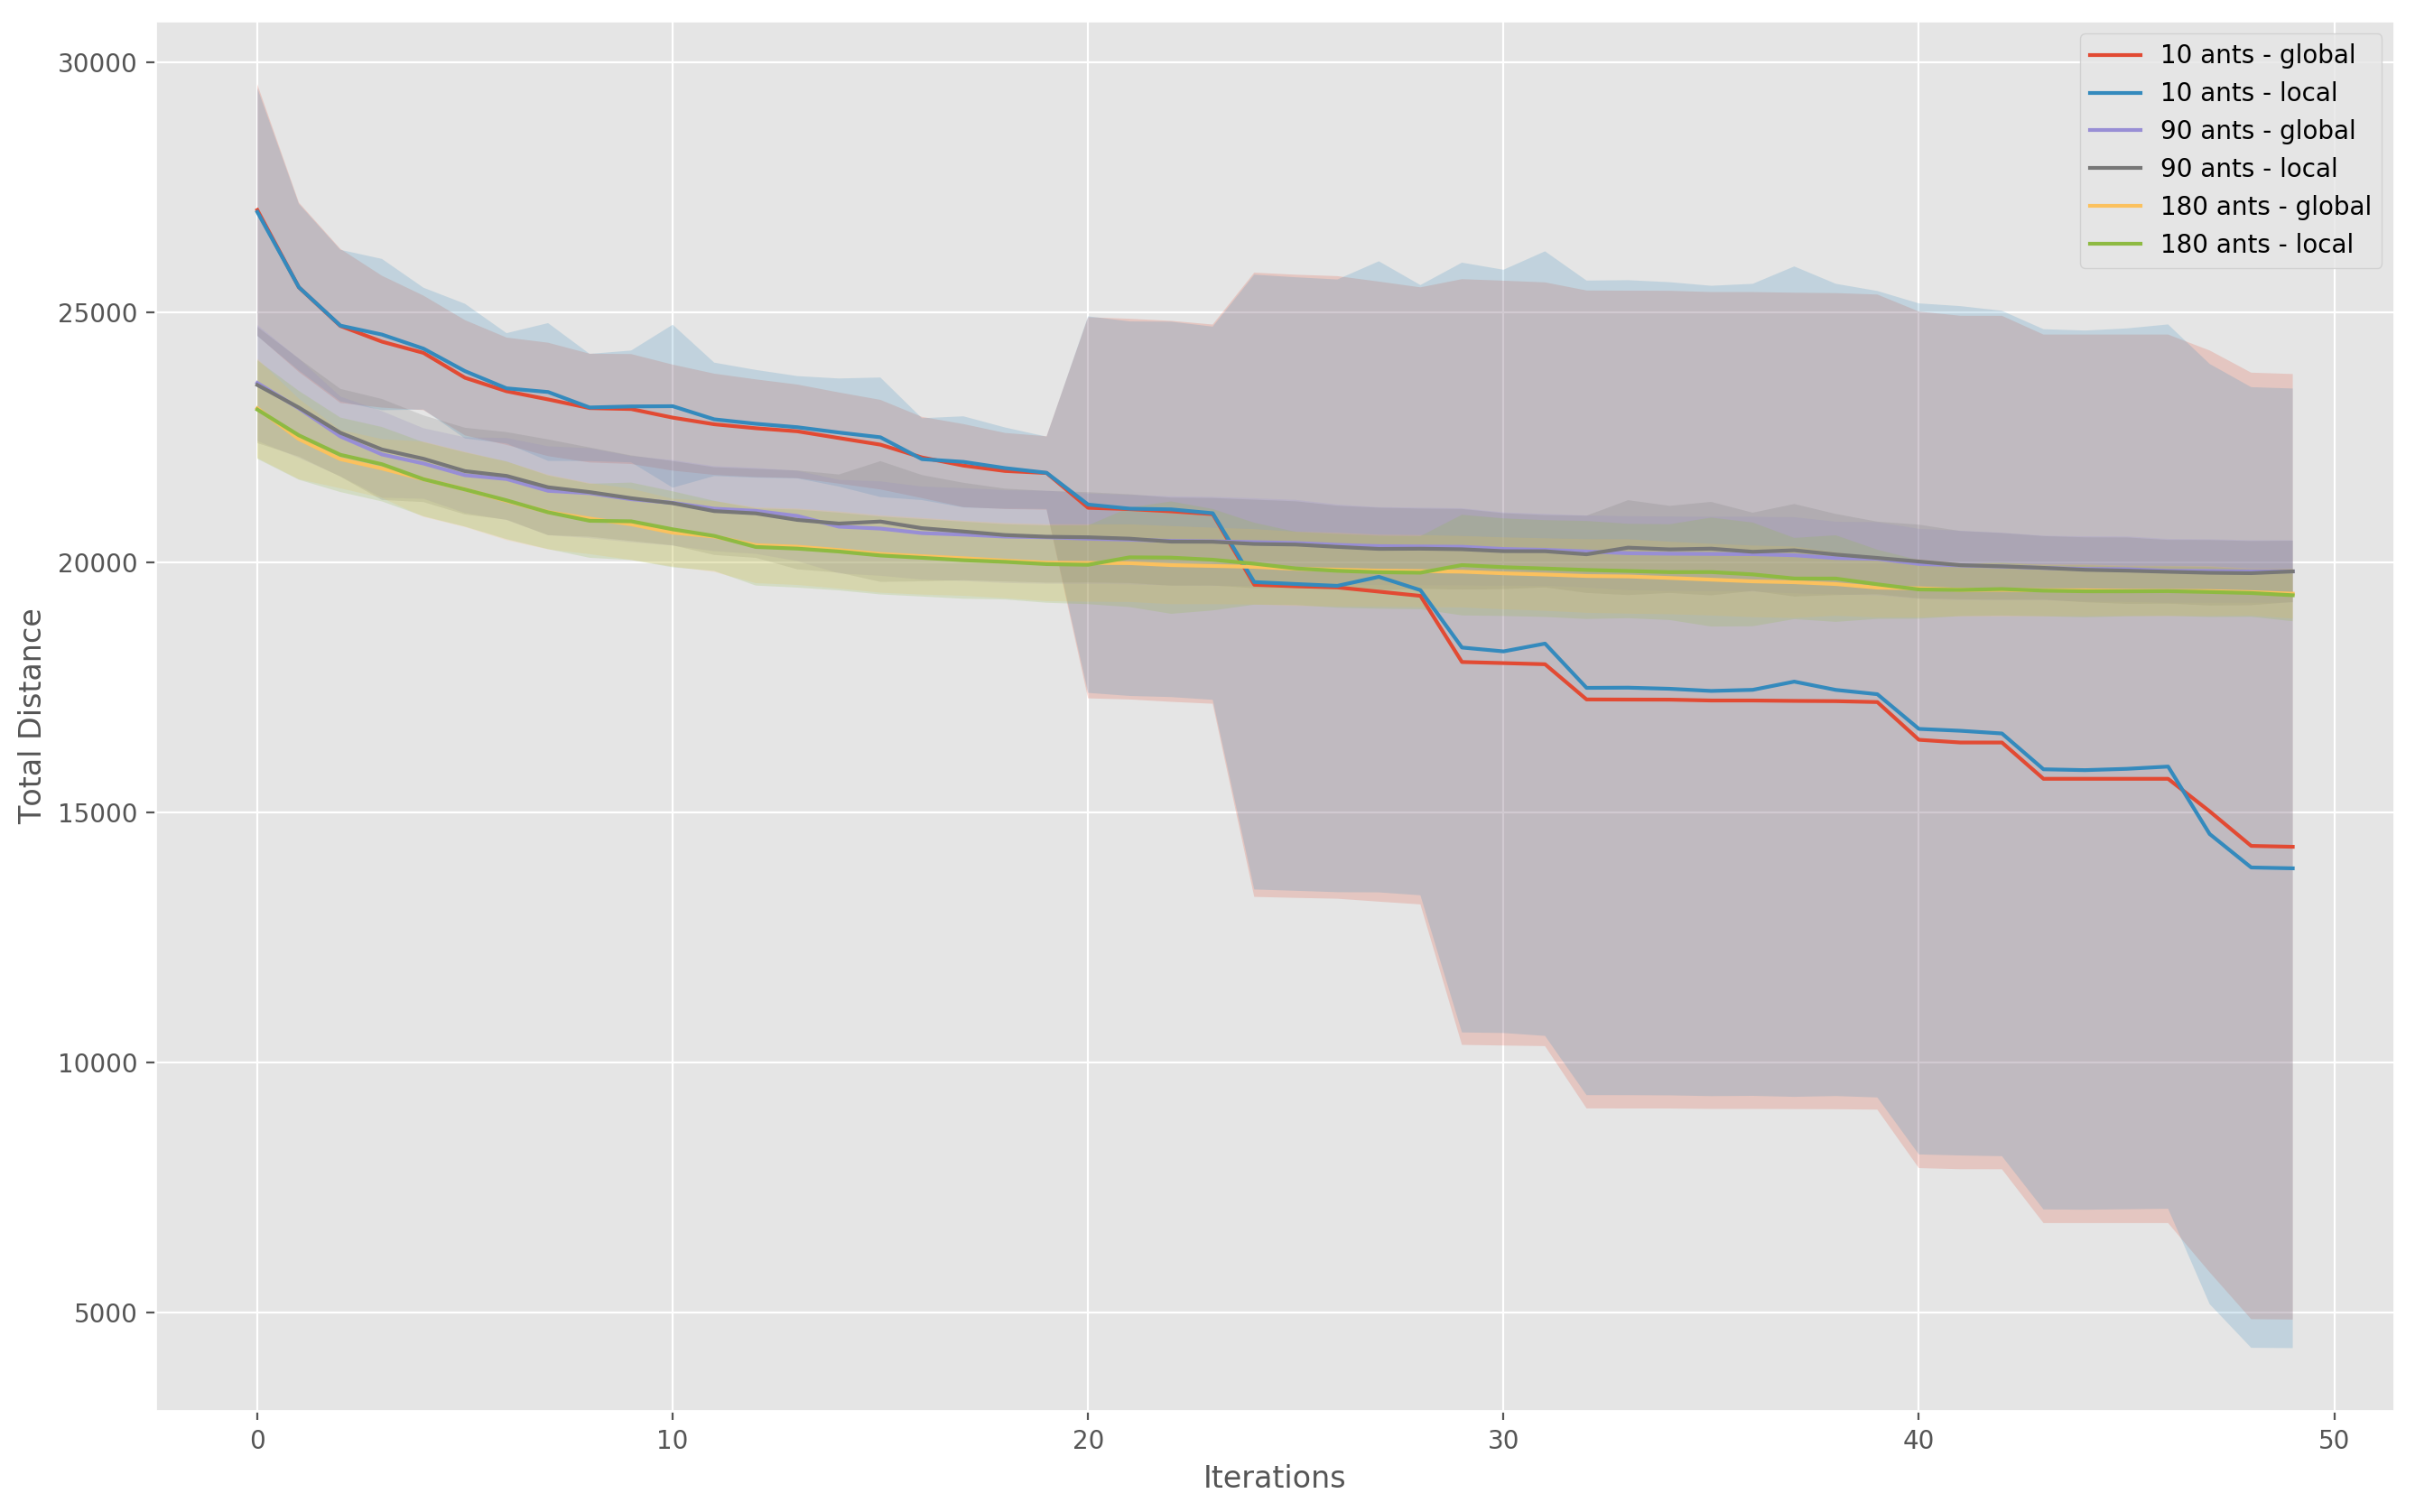
\includegraphics[width=11cm,keepaspectratio]{images/SJC1_ants.png}
  \caption{Média e desvio padrão para a distância da solução encontrada para base SJC1 com número de formigas variável.}
  \label{fig:sjc1_ants}
\end{figure}

Em seguida avaliamos os efeitos da variação da taxa de evaporação do feromônio($\rho$). Na Figura \ref{fig:sjc1_rho} vemos algo peculiar: os valores 0, 0.1 e 0.5 para a $\rho$ se sobrepõem no gráfico, pois geram exatamente os mesmos resultados. Como a evaporação do feromônio é muito sutil, o que provavelmente acontece é que o resultado do termo $\rho(\Delta\tau_i - \tau_i)$ fica muito pequeno a ponto de se tornar irrelevante para levar as soluções para outro caminho, ou seja, o espaço de soluções é mal explorado. O melhor valor para $\rho$ encontrado foi \textbf{0.99}. Com $\rho \geq 1$ o algoritmo não consegue progredir.

\begin{figure}[h]	
  \centering
  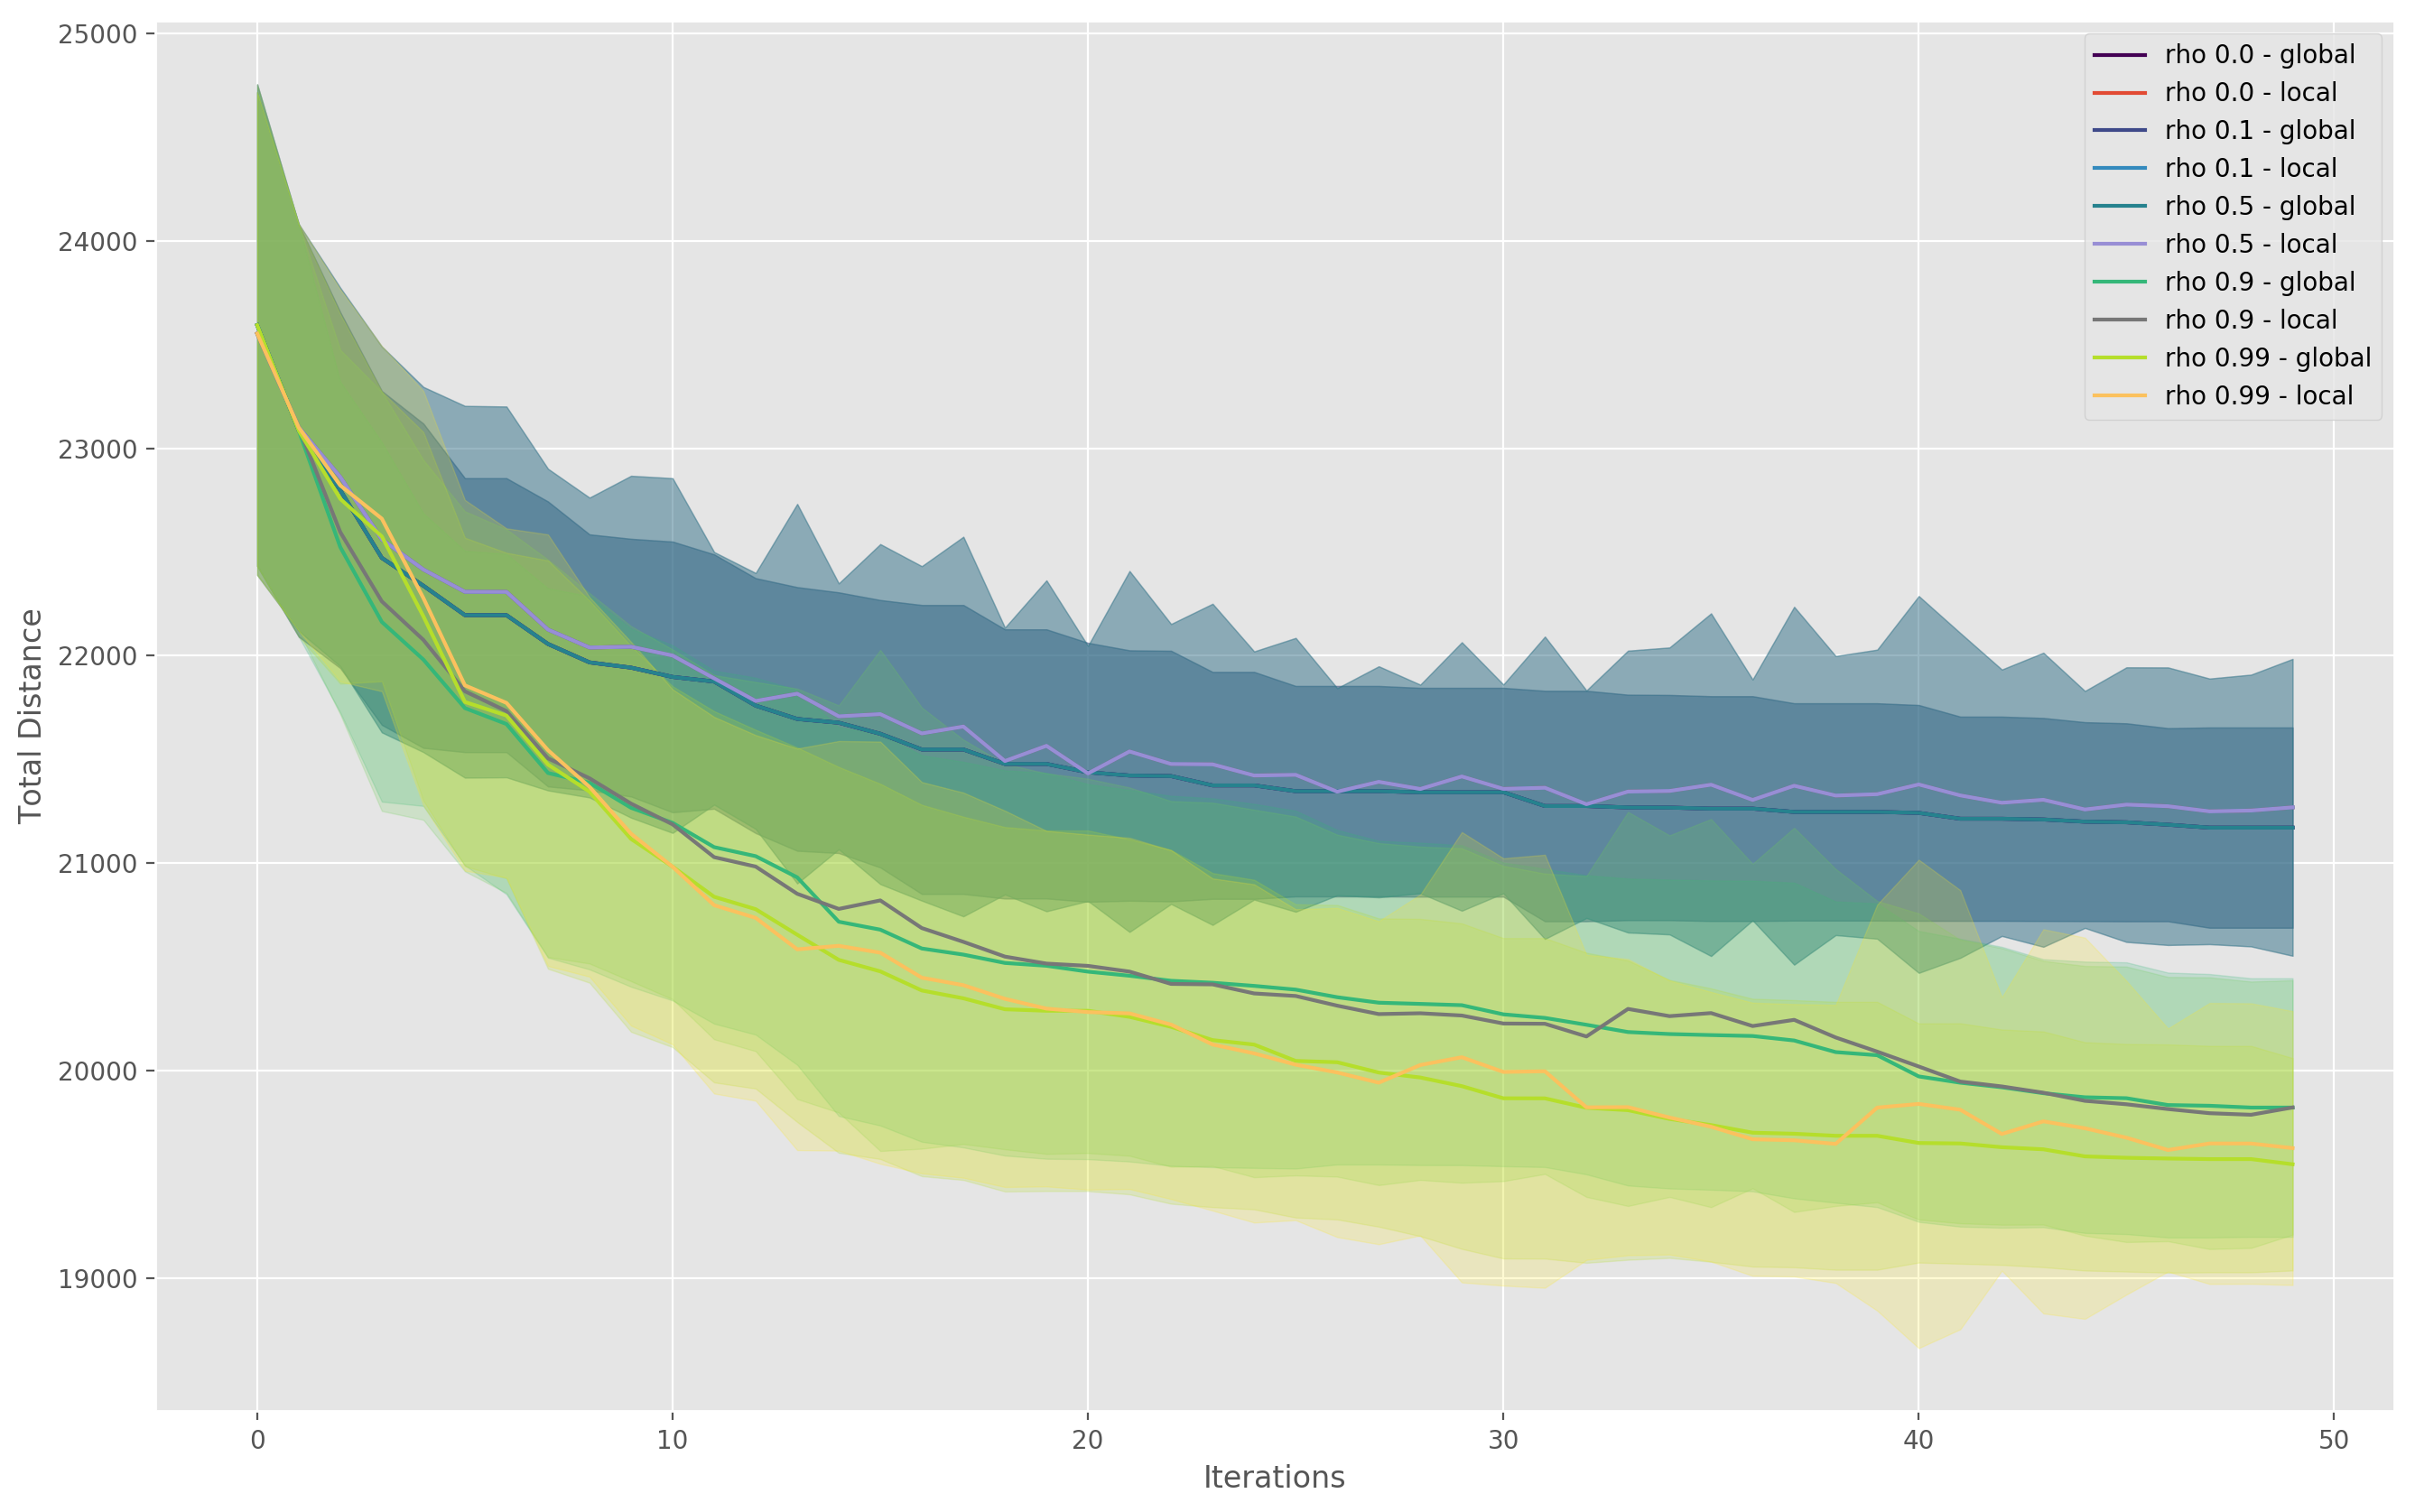
\includegraphics[width=11cm,keepaspectratio]{images/SJC1_rho.png}
  \caption{Média e desvio padrão para a distância da solução encontrada para base SJC1 com taxa de evaporação de feromônio variável.}
  \label{fig:sjc1_rho}
\end{figure}

Como última variação vamos analisar a influência dos indicadores $\alpha$ e $\beta$. Pelo gráfico na Figura \ref{fig:sjc1_alpha_beta} podemos ver que, apesar de a média do melhor global para $\alpha = 3$ e $\beta = 1$ ser melhor que a média do melhor local para $\alpha = 1$ e $\beta = 0$, a média global do último é melhor, o que contra o padrão dos resultados de \cite{de2005max}.

\begin{figure}[h]	
  \centering
  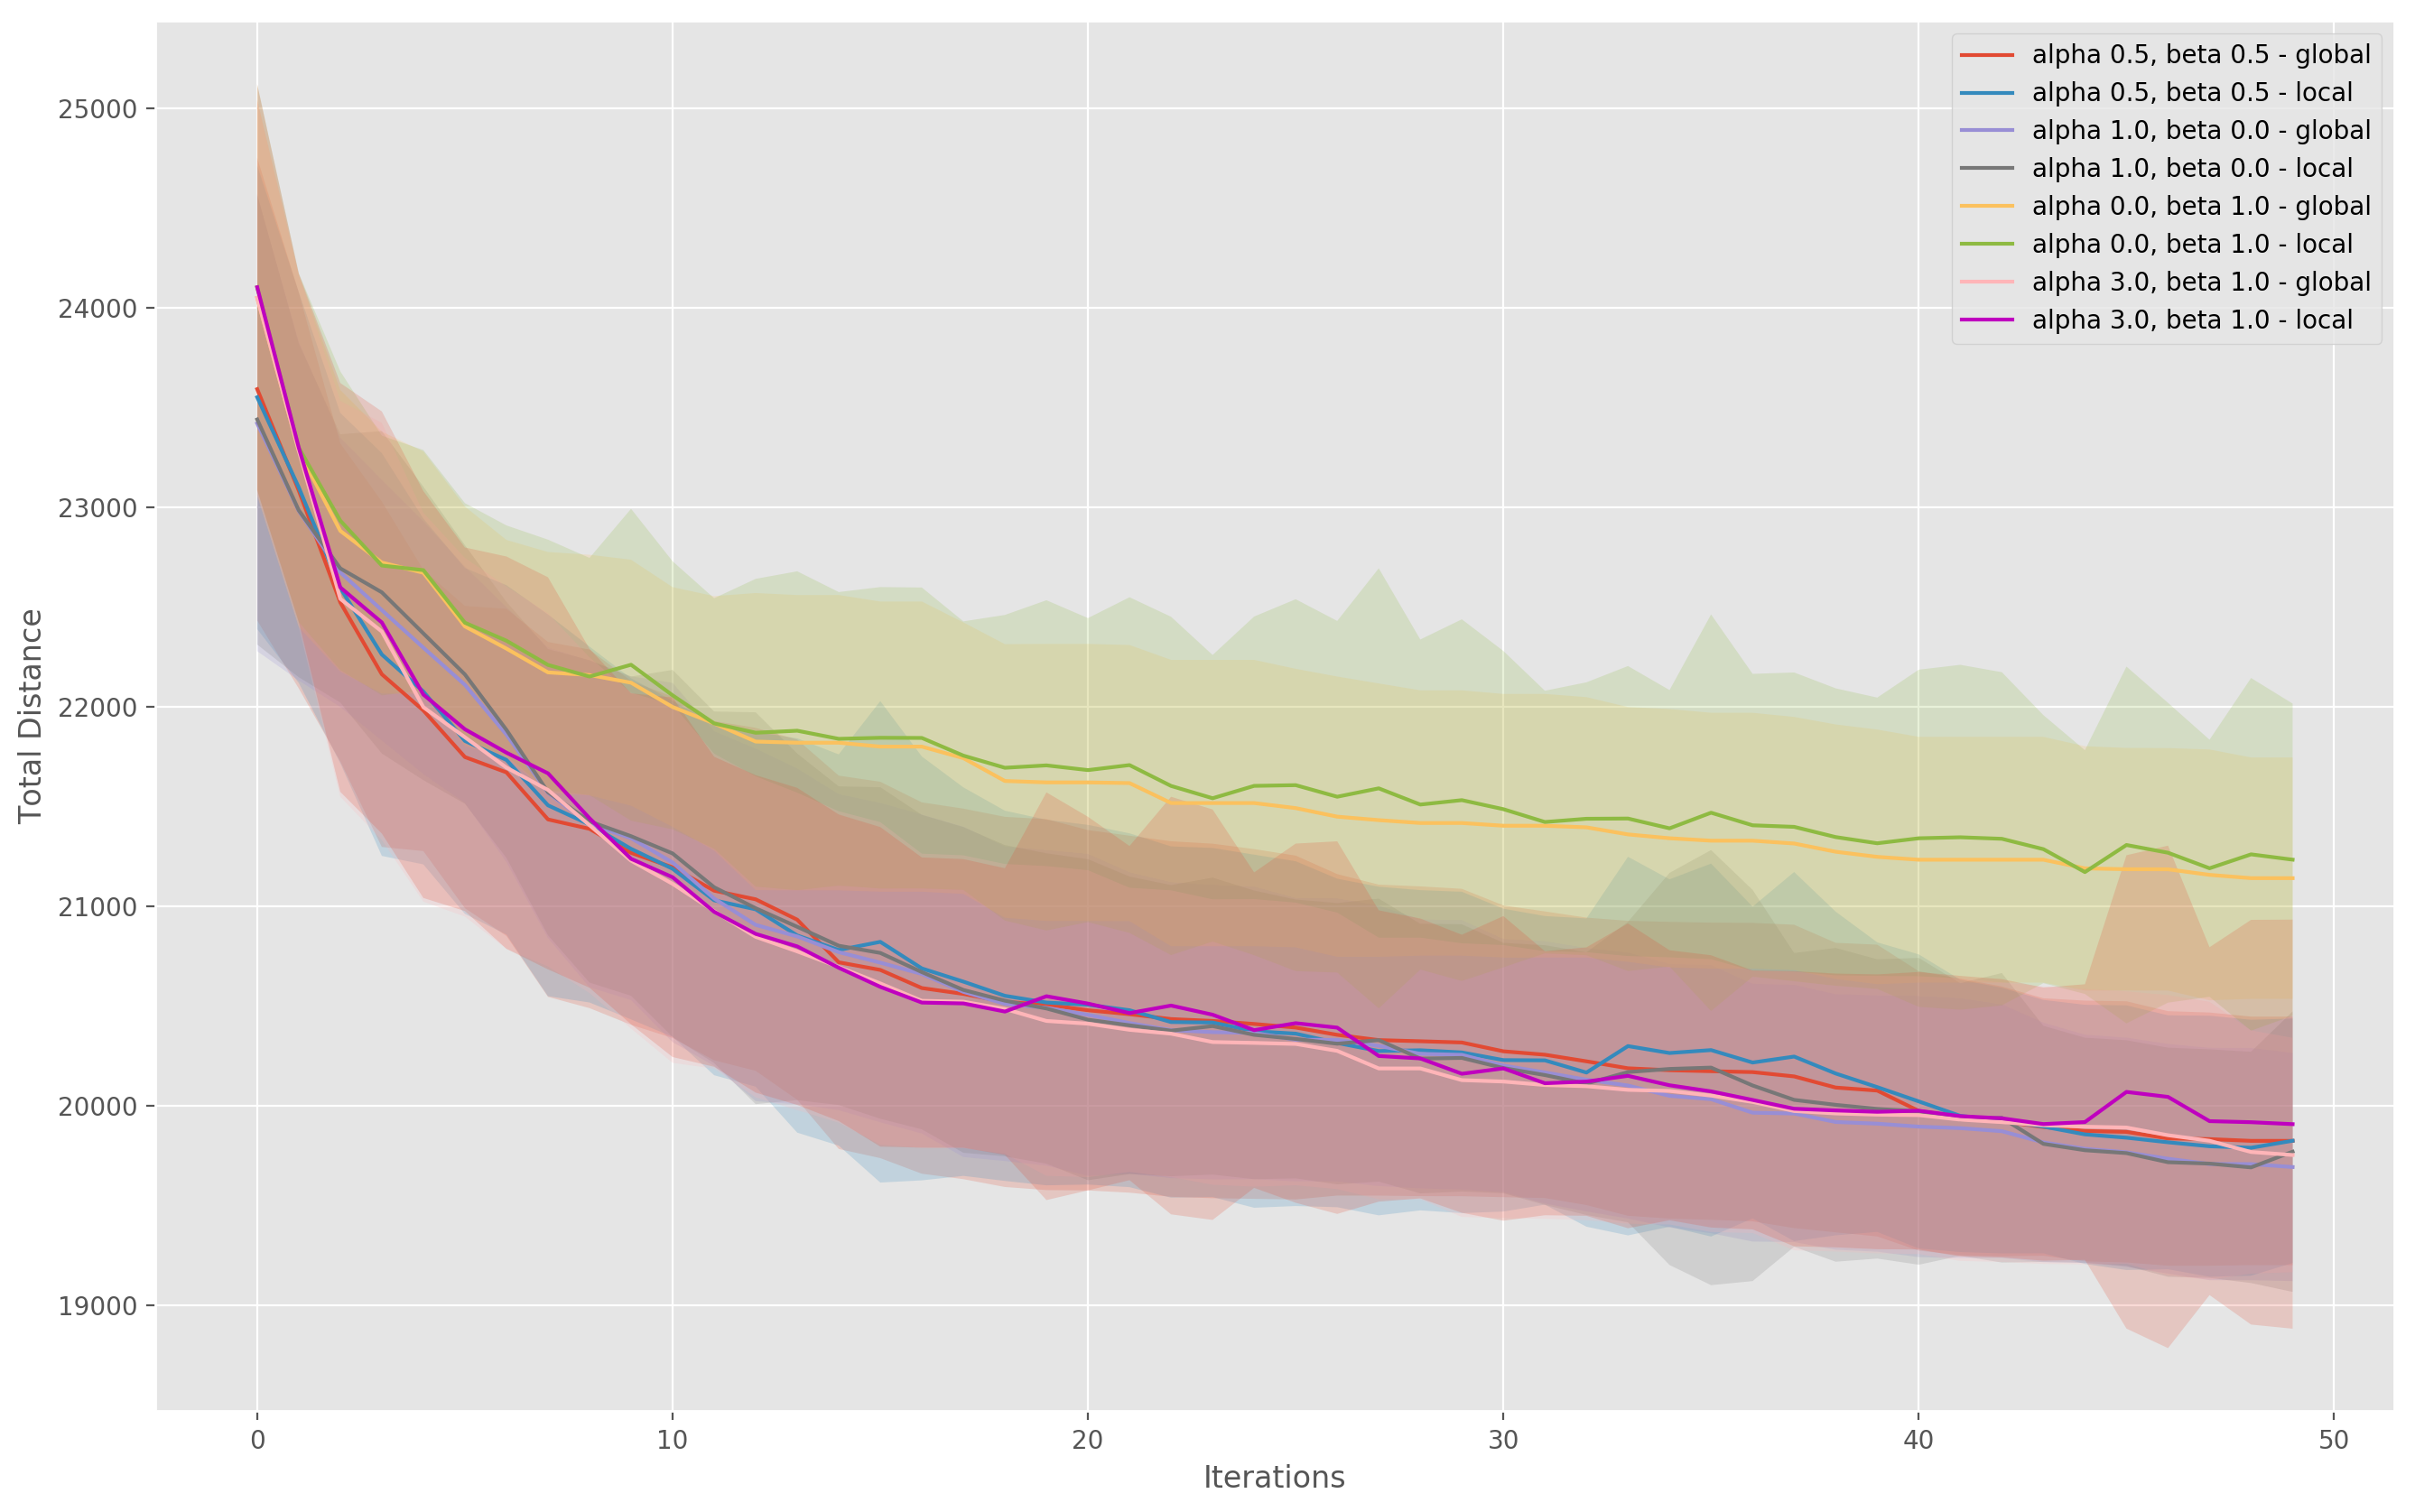
\includegraphics[width=11cm,keepaspectratio]{images/SJC1_alpha_beta.png}
  \caption{Média e desvio padrão para a distância da solução encontrada para base SJC1 com a variação dos pesos dos feromônios e da heurística de informação no cálculo da probabilidade de escolha do nó.}
  \label{fig:sjc1_alpha_beta}
\end{figure}

Por fim mostramos na Figura \ref{fig:sjc1_best} o melhor resultado encontrado entre as repetições para todas as variações de parâmetros testadas até agora. A melhor combinação de parâmetros foi 100 iterações, 180 formigas, $\rho = 0.99$, $\alpha=1$ e $\beta=0$ Ignorando a execução problemática, a combinação dos melhores parâmetros encontrados até agora foi a que performou melhor, alcançando, na melhor das repetições, uma distância total de \textbf{18009.965} entre os clientes e os centros. 

\begin{figure}[h]	
  \centering
  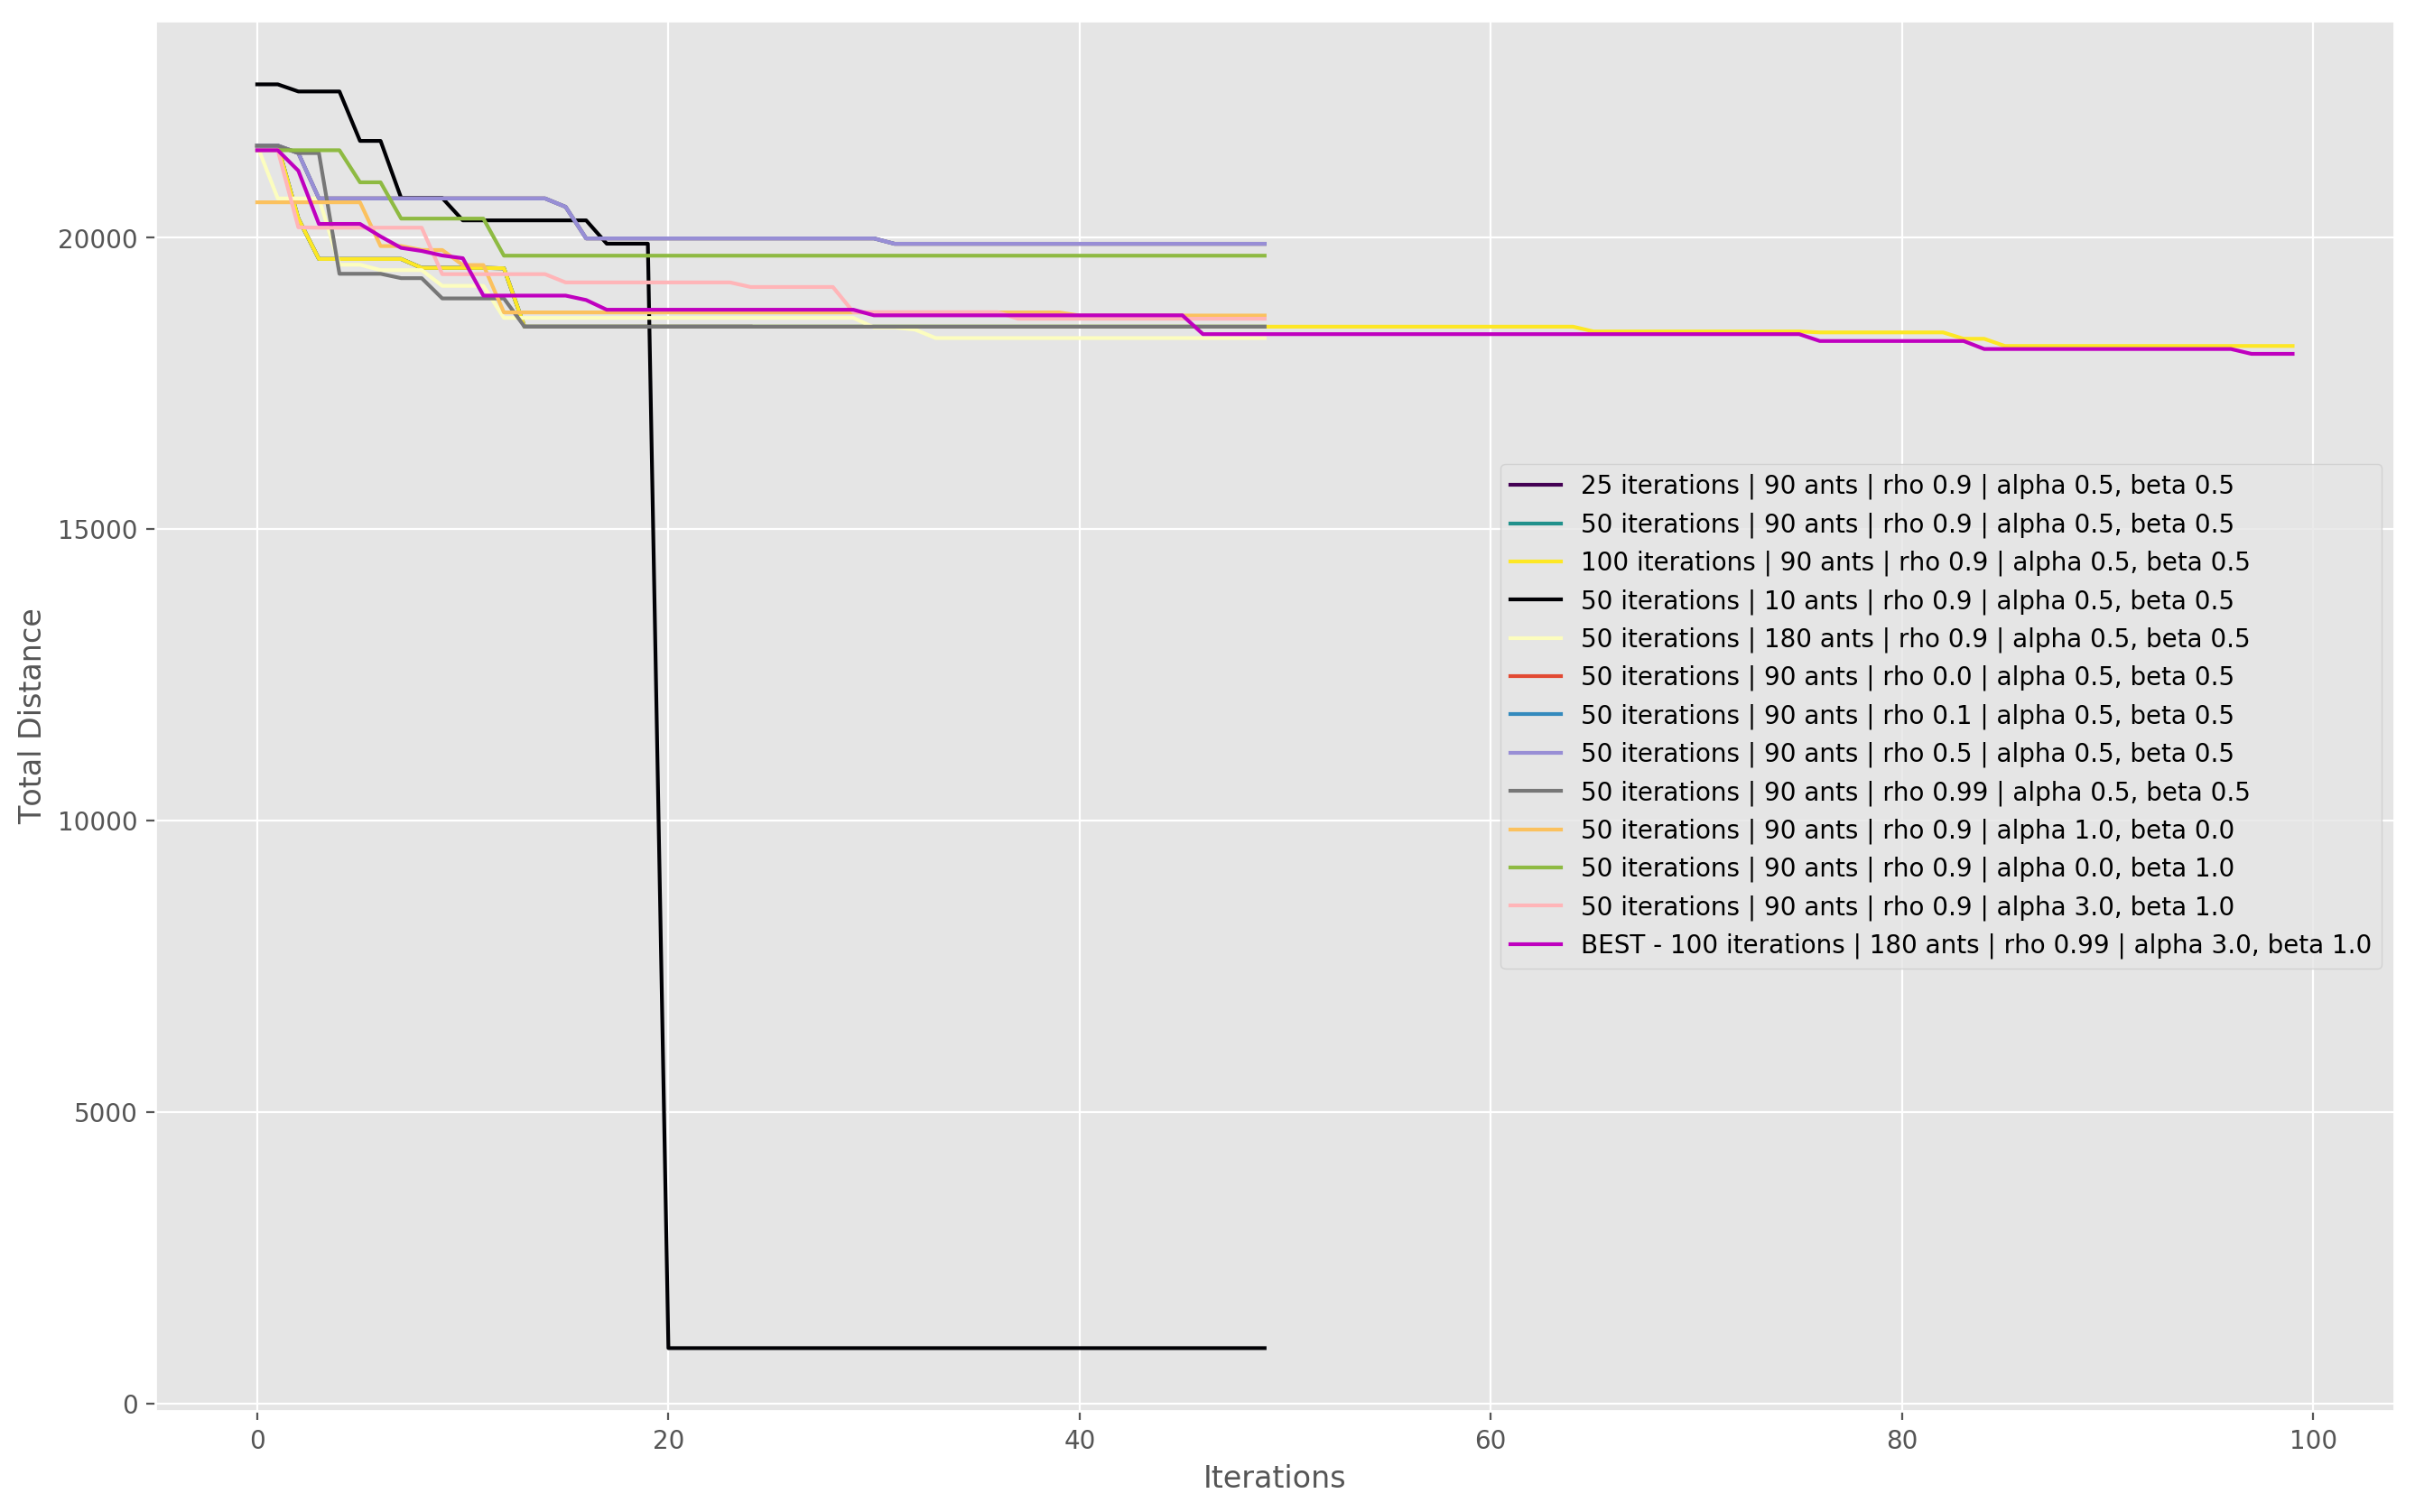
\includegraphics[width=11cm,keepaspectratio]{images/SJC1_best.png}
  \caption{Melhores soluções encontradas para a base SJC1 ao longo das repetições para todas as variações de parâmetros apresentadas até agora.}
  \label{fig:sjc1_best}
\end{figure}



\subsubsection{SJC2}

A base de dados SJC2 é composta de 200 pontos, todos com capacidade 840, mas com demanda variável. Ela busca por 15 pontos de mediana. Novamente vamos começar avaliando os resultados gerados para diferentes números de gerações. Em realidade, a análise experimental para essa base se dará com a mesma estrutura da base anterior, assim como ocorrerá com a base seguinte. Aqui, novamente o maior número de iterações se mostrou superior, como visto na Figura \ref{fig:sjc2_iterations}.

\begin{figure}[h]	
  \centering
  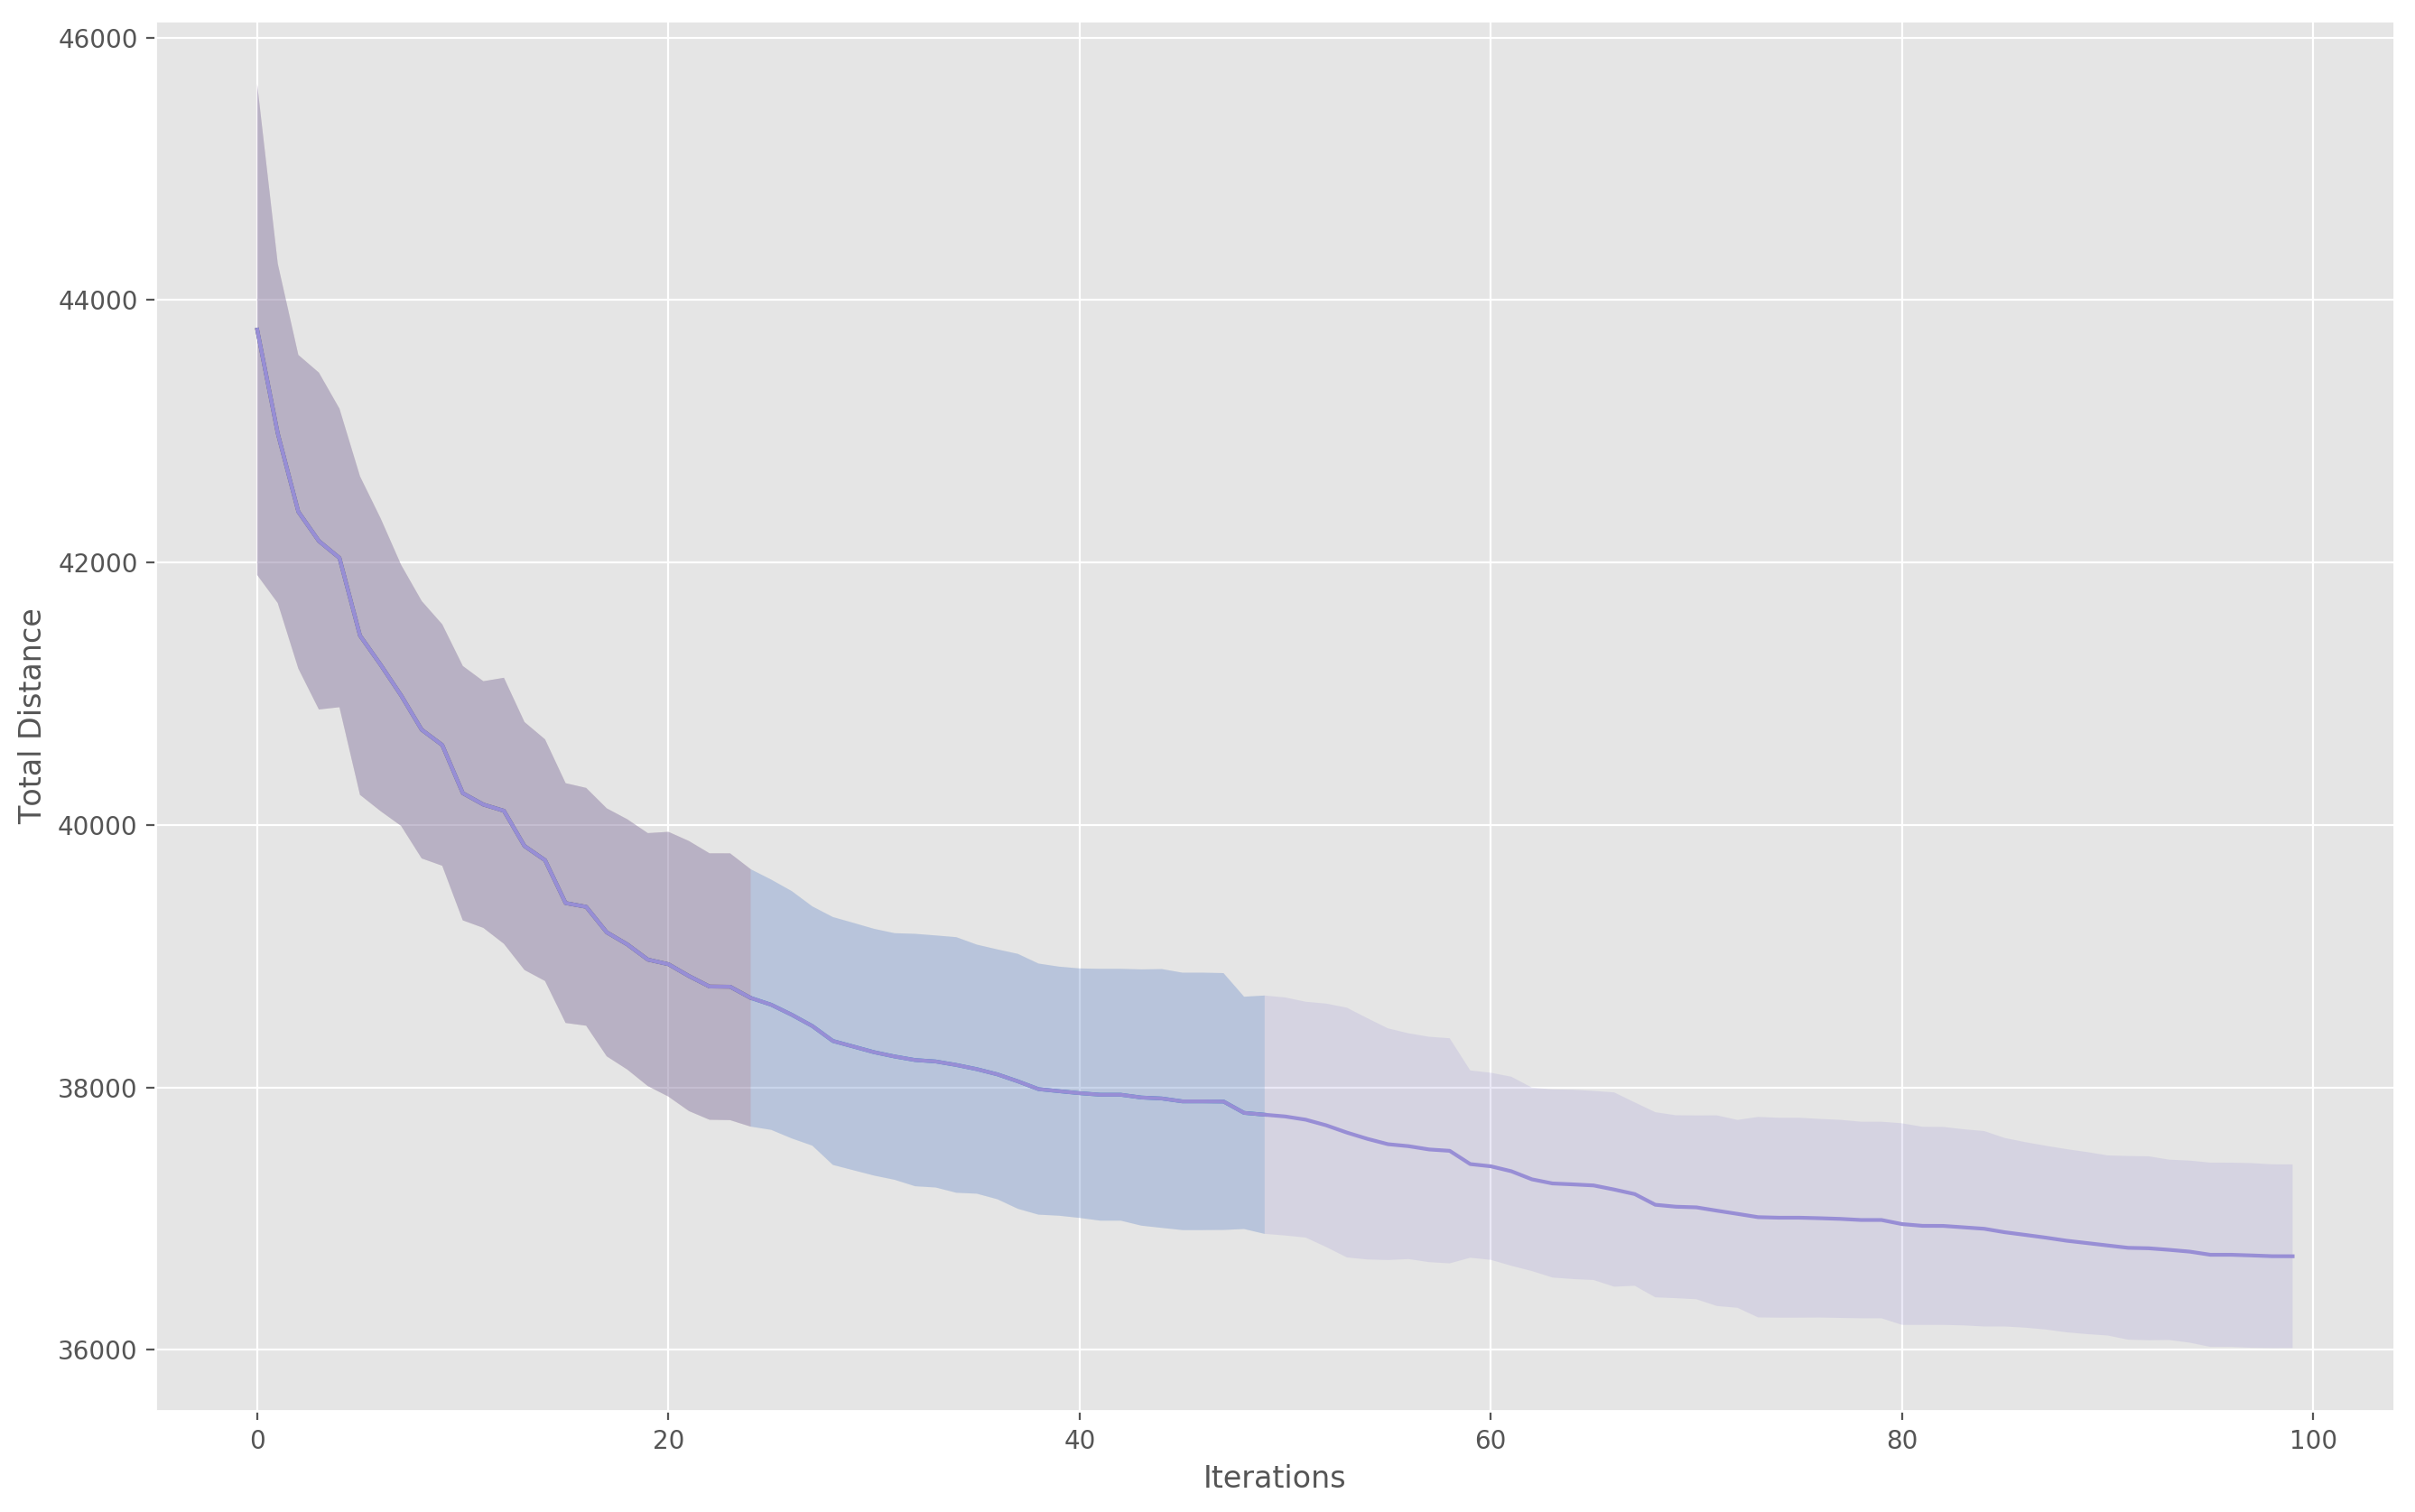
\includegraphics[width=11cm,keepaspectratio]{images/SJC2_iterations.png}
  \caption{Média e desvio padrão para a distância da solução encontrada para base SJC2 com número de iterações variável.}
  \label{fig:sjc2_iterations}
\end{figure}

Ao variarmos o número de formigas na colônia também encontramos resultados semelhantes à base SCJ1, com $2 * (n - p)$ formigas se mostrando mais eficiente. Os resultados estão na Figura \ref{fig:sjc2_ants}.

\begin{figure}[h]	
  \centering
  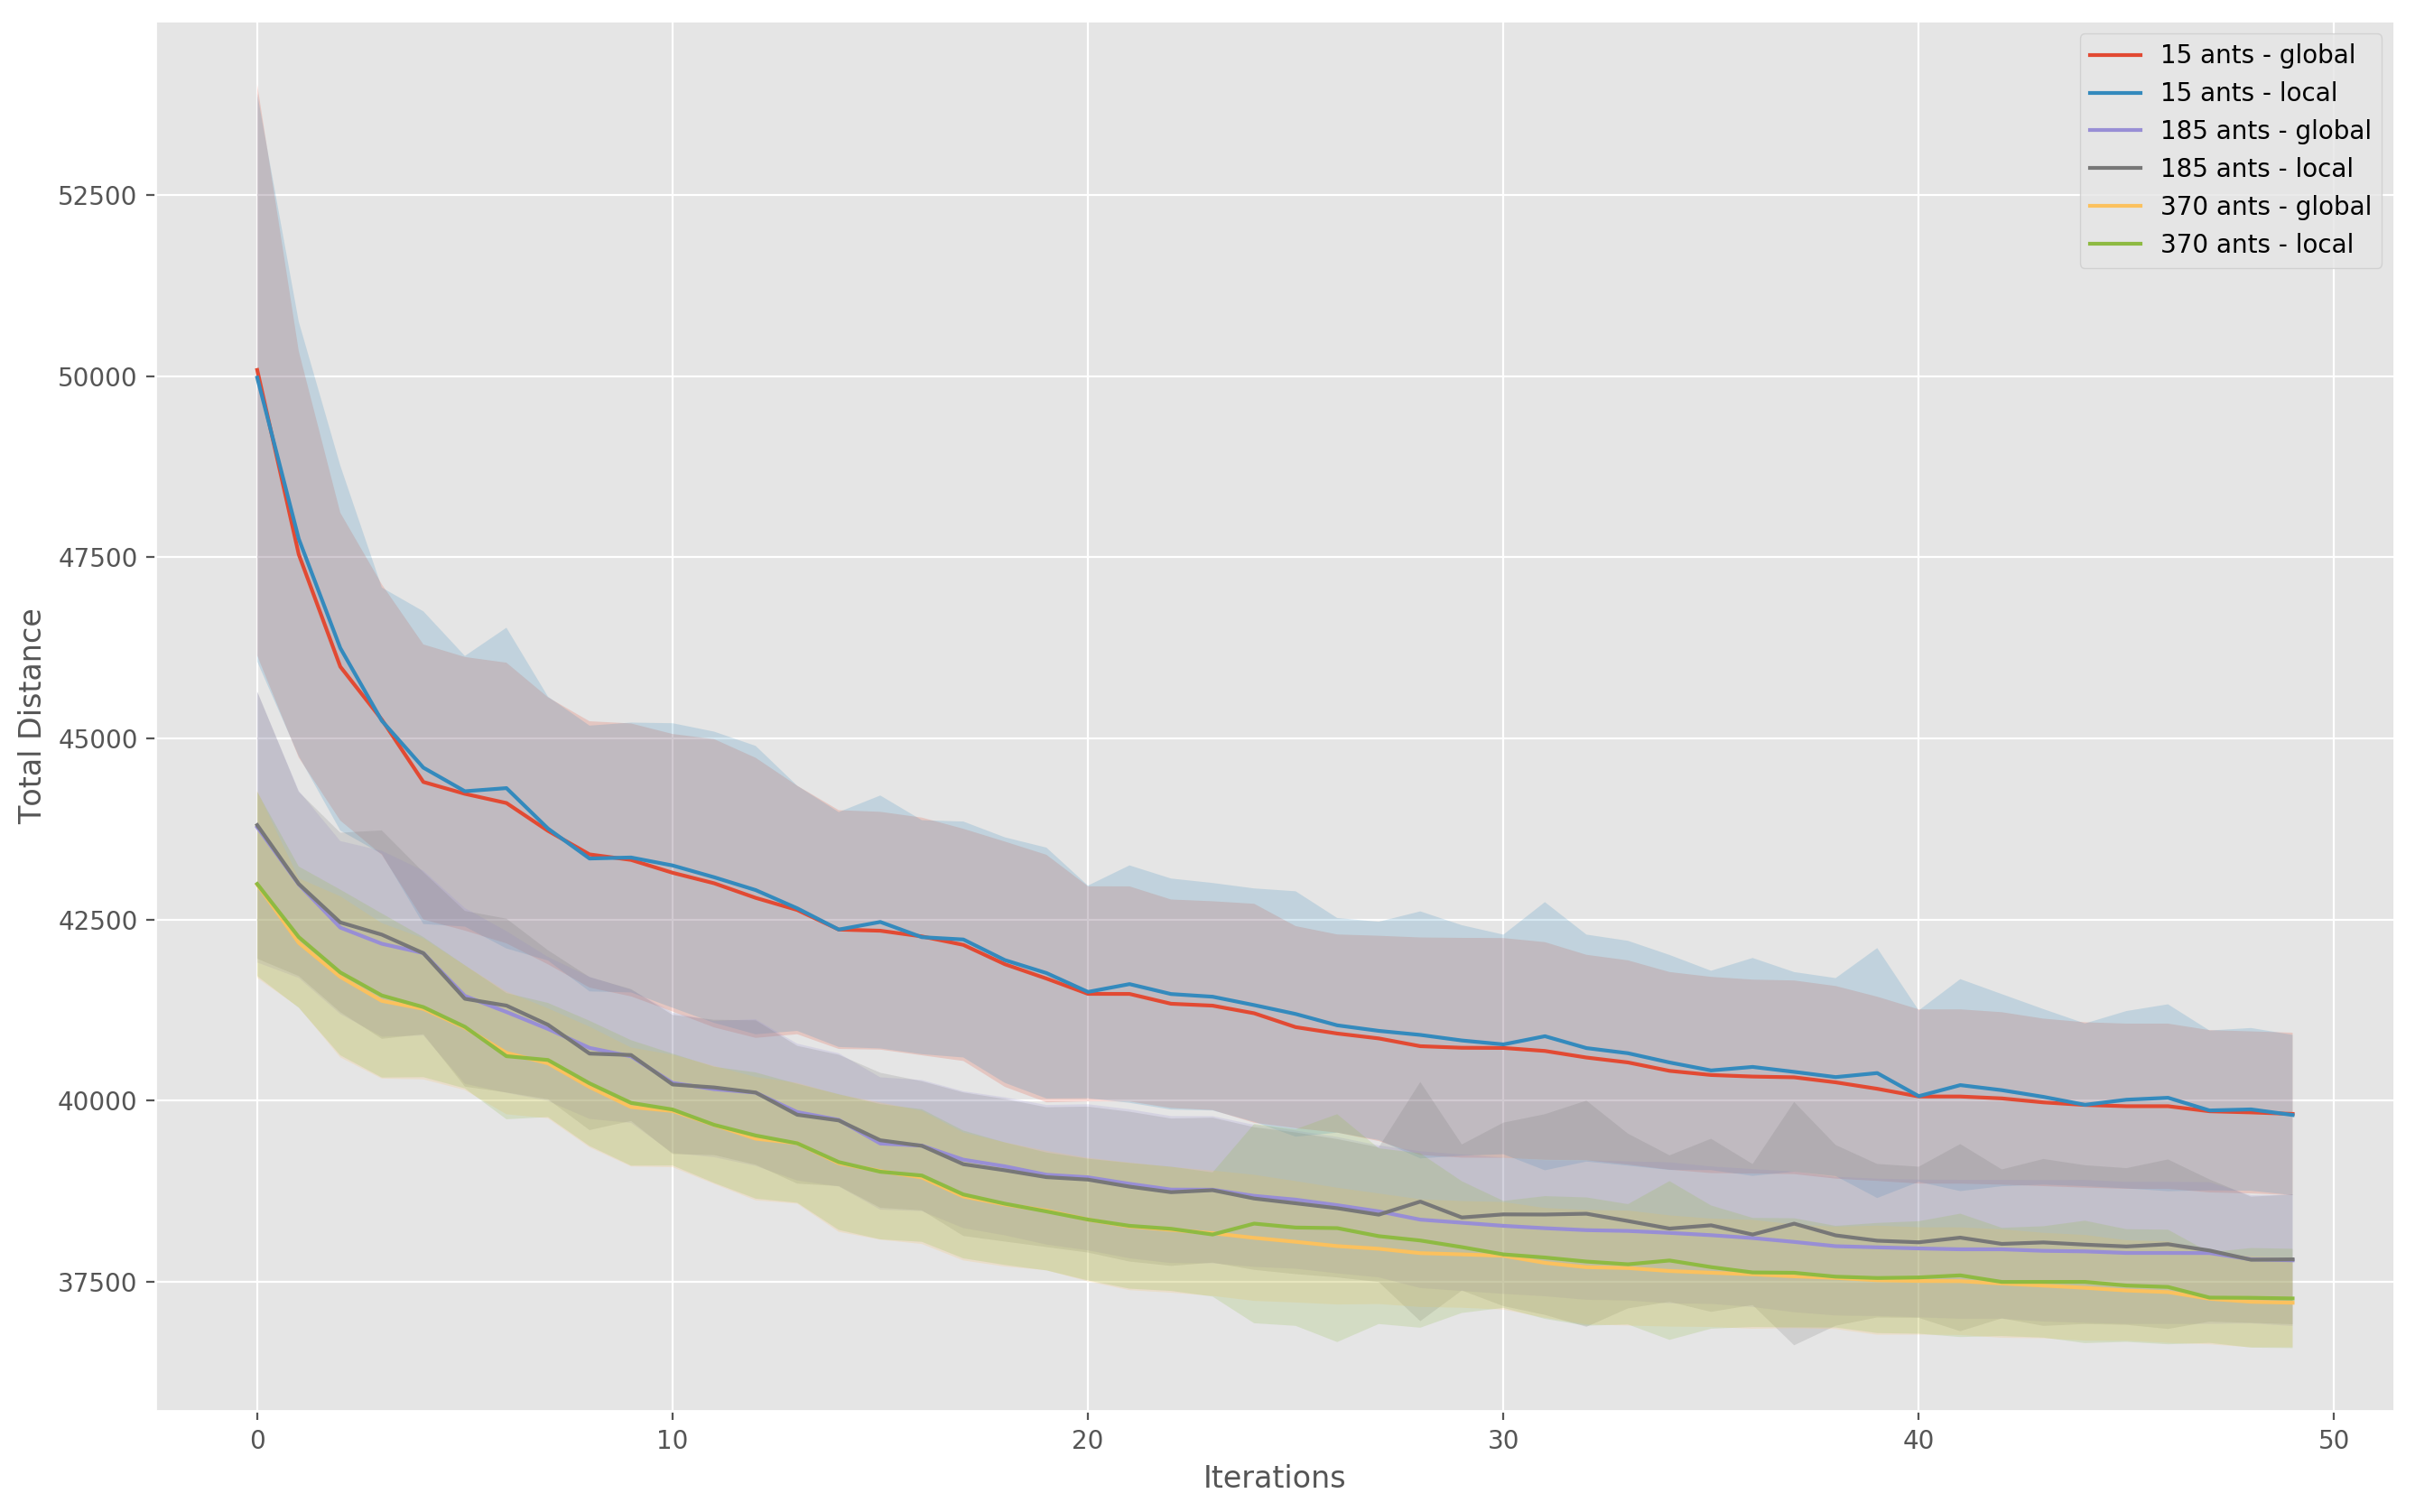
\includegraphics[width=11cm,keepaspectratio]{images/SJC2_ants.png}
  \caption{Média e desvio padrão para a distância da solução encontrada para base SJC2 com número de formigas variável.}
  \label{fig:sjc2_ants}
\end{figure}

Com relação ao termo $\rho$ encontramos um cenário idêntico ao da base anterior, como é possível ver na Figura \ref{fig:sjc2_rho}, ou seja, o valor ótimo é $\rho = 0.99$. 

\begin{figure}[h]	
  \centering
  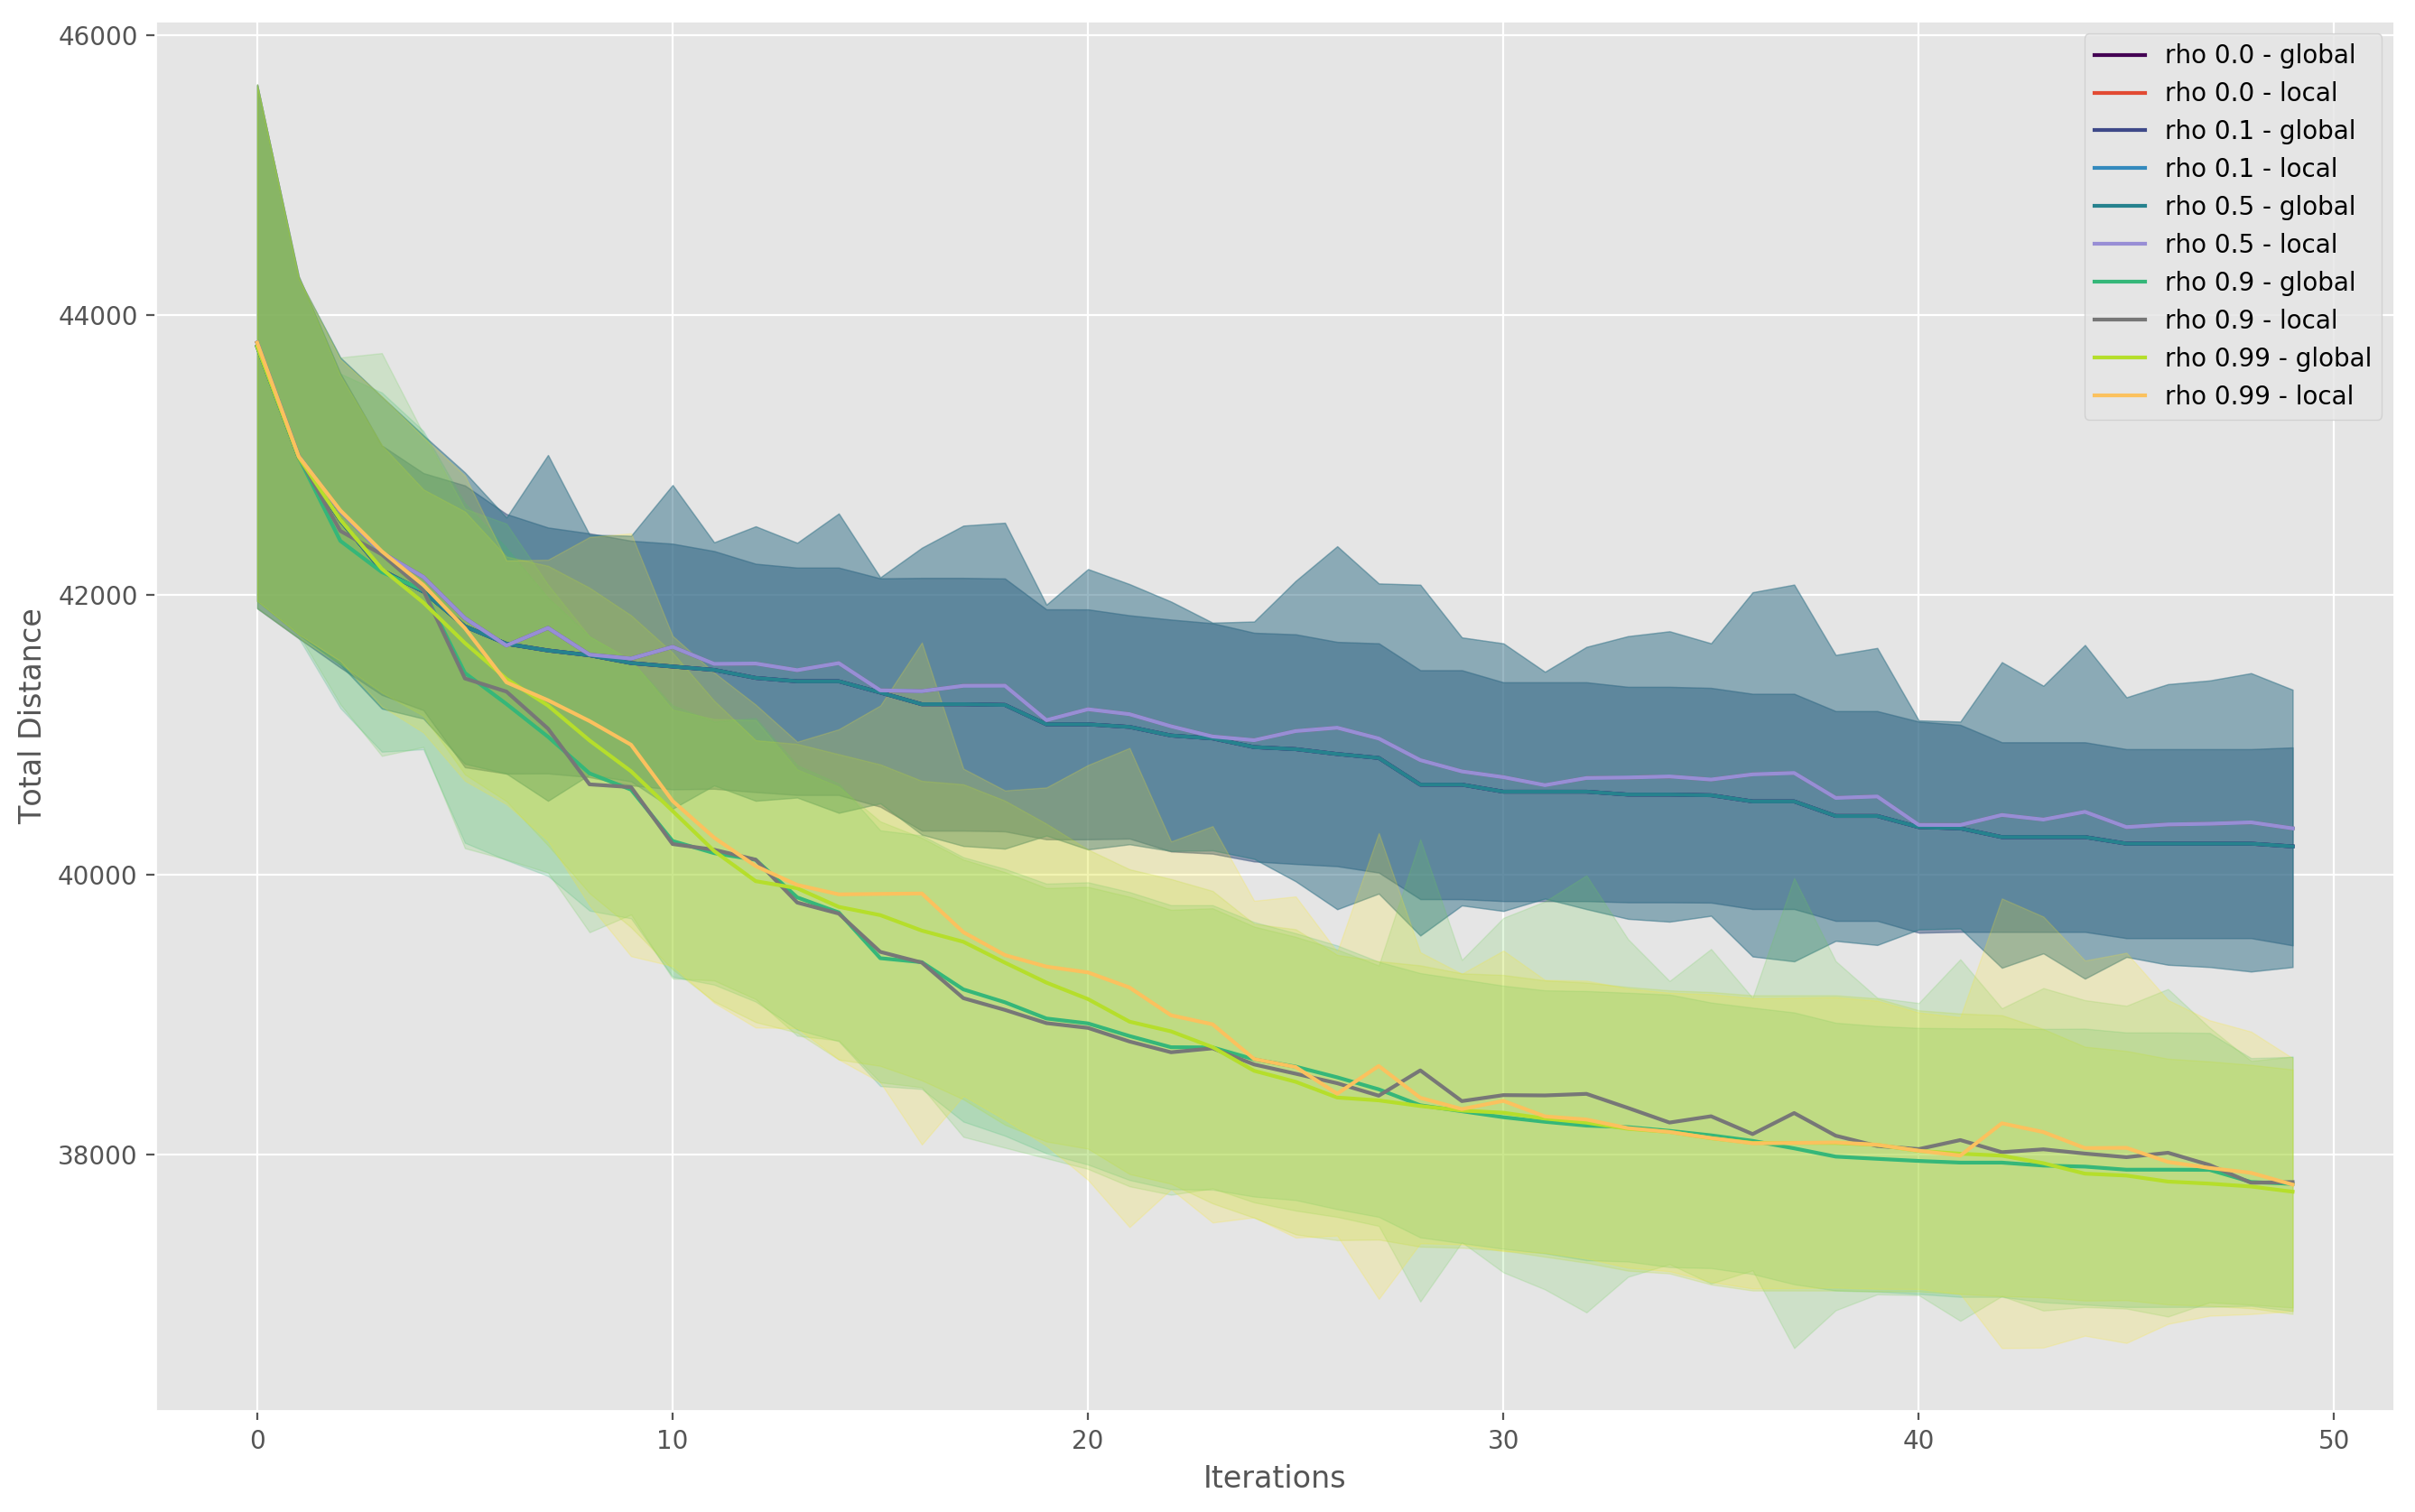
\includegraphics[width=11cm,keepaspectratio]{images/SJC2_rho.png}
  \caption{Média e desvio padrão para a distância da solução encontrada para base SJC2 com taxa de evaporação de feromônio variável.}
  \label{fig:sjc2_rho}
\end{figure}

Para os termos $\alpha$ e $\beta$ temos um resultado semelhante ao anterior: os valores ótimos são indubitavelmente $\alpha=1$ e $\beta=0$, o que vai novamente contra os resultados em \cite{de2005max}.

\begin{figure}[h]	
  \centering
  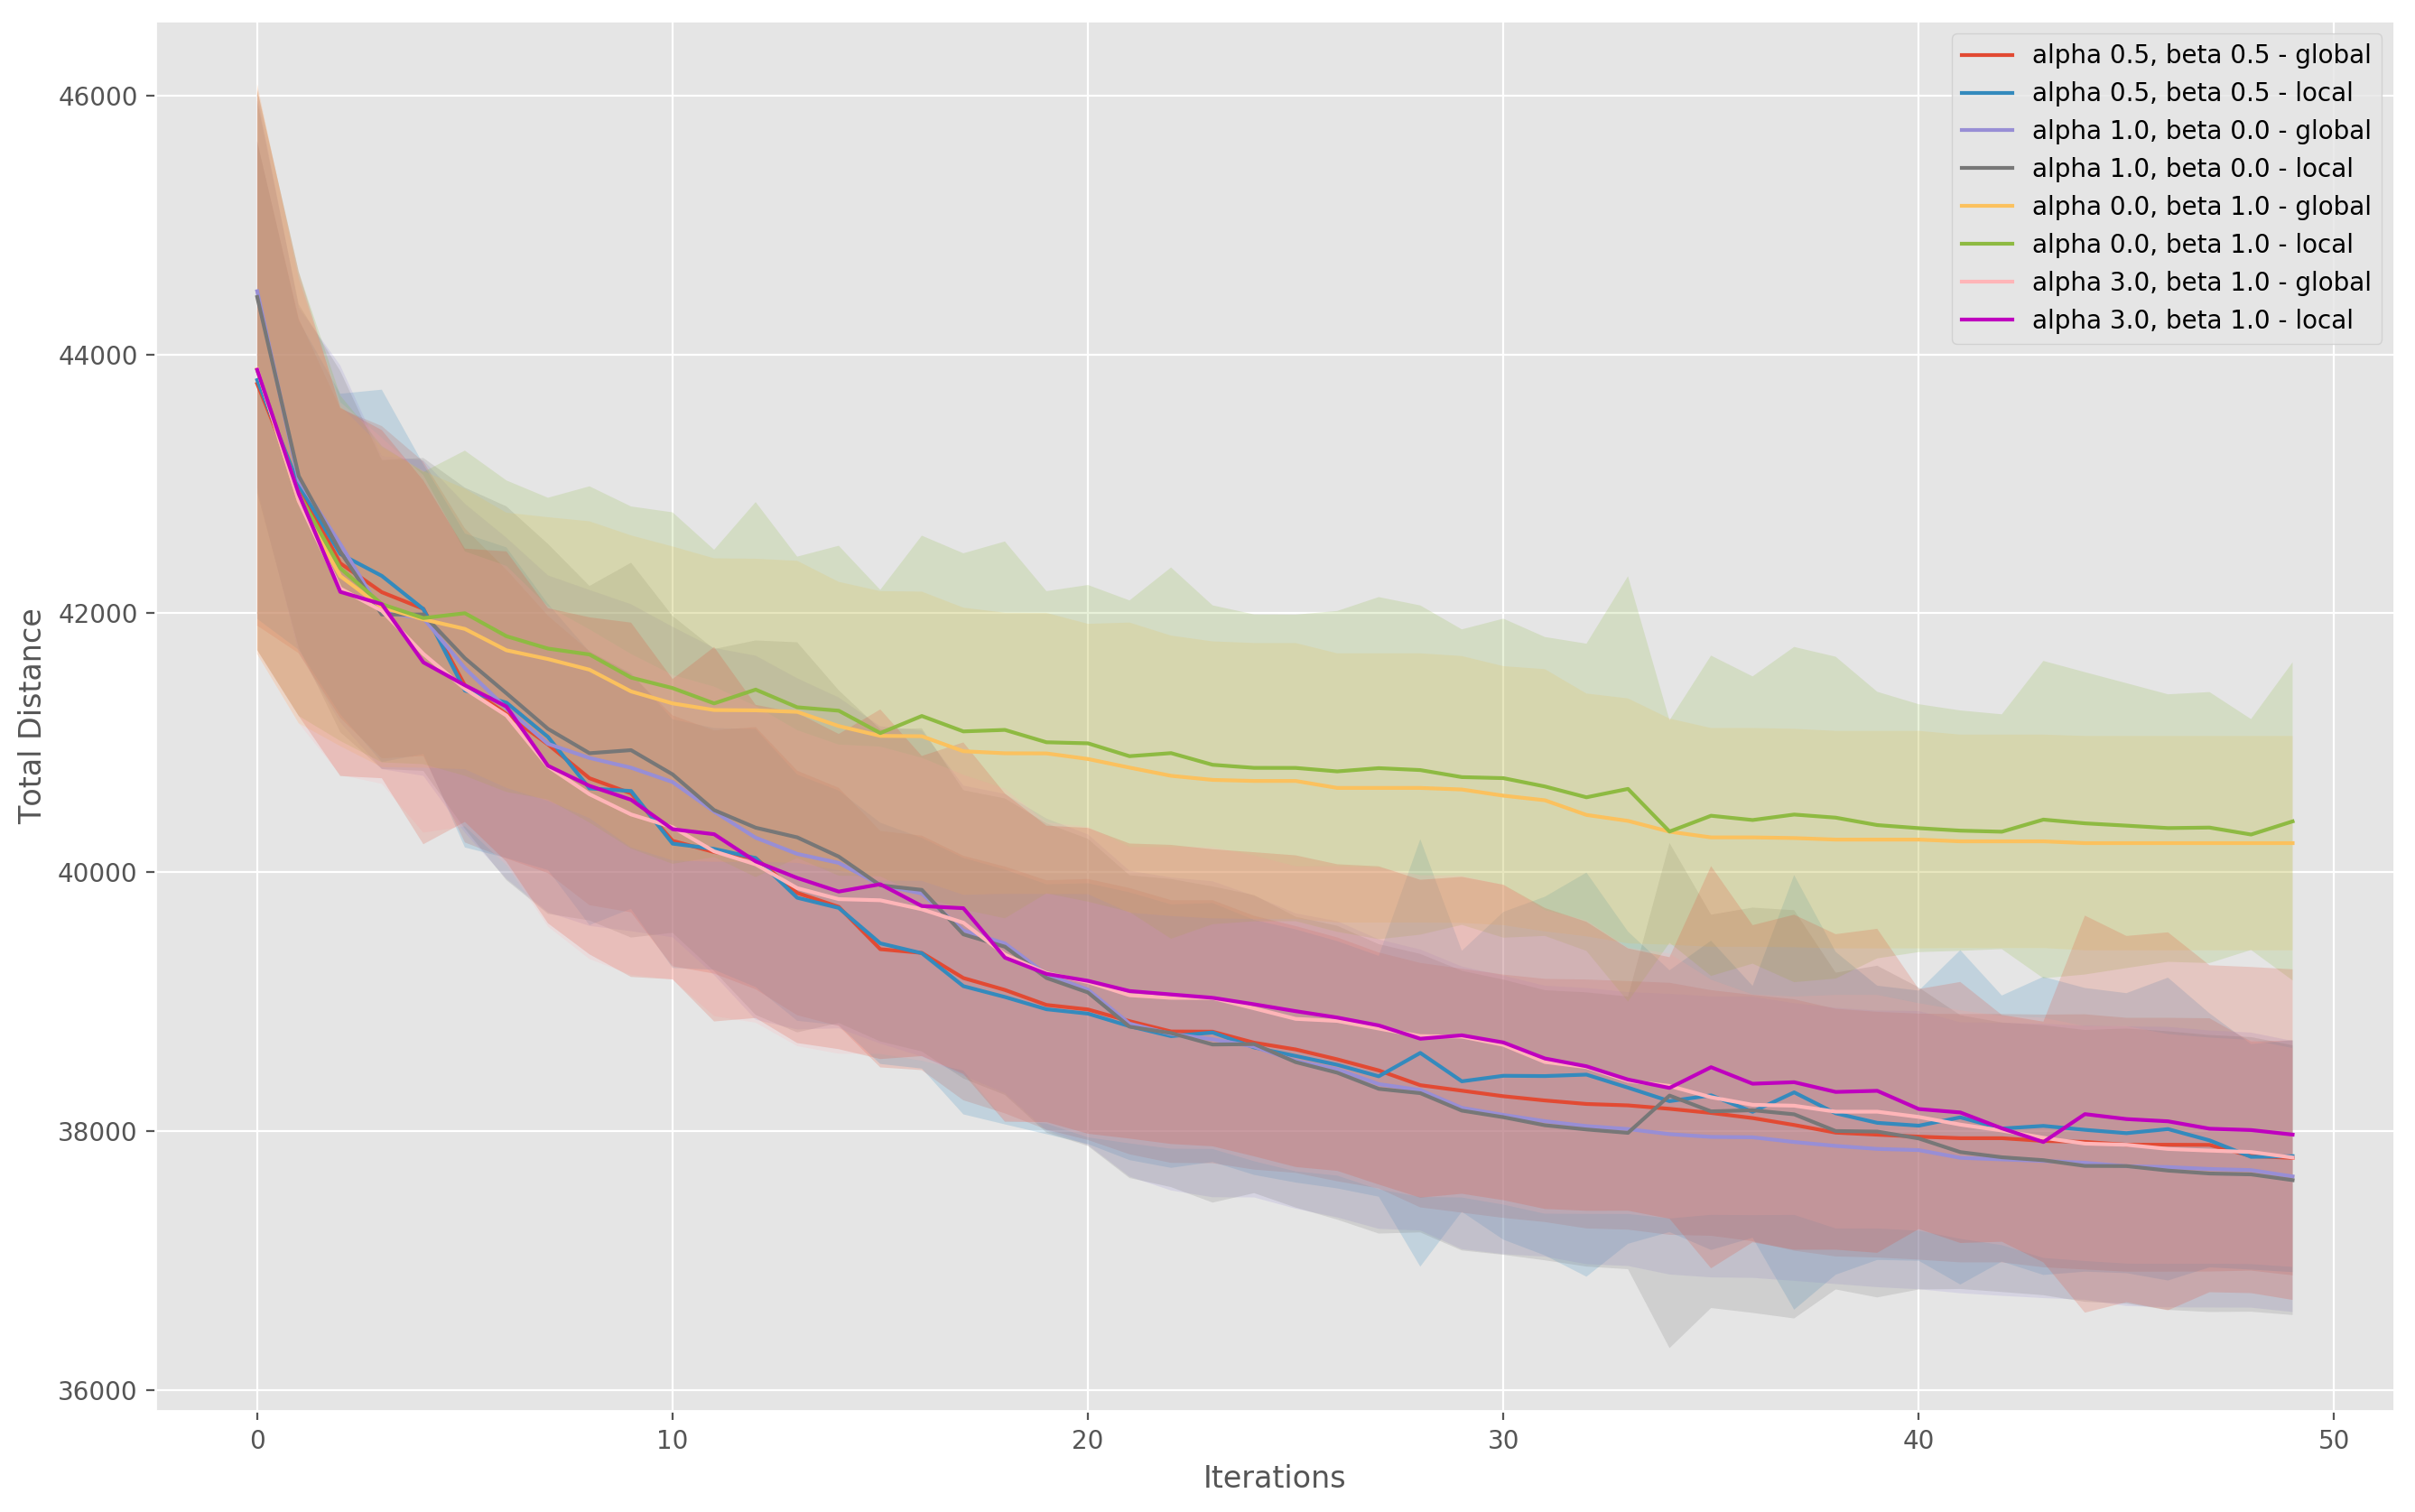
\includegraphics[width=11cm,keepaspectratio]{images/SJC2_alpha_beta.png}
  \caption{Média e desvio padrão para a distância da solução encontrada para base SJC2 com a variação dos pesos dos feromônios e da heurística de informação no cálculo da probabilidade de escolha do nó.}
  \label{fig:sjc2_alpha_beta}
\end{figure}

Juntos, os melhores parâmetros encontrados foram 100 iterações, 370 formigas, $\rho = 0.99$, $\alpha=1$ e $\beta=0$. Na Figura \ref{fig:sjc2_best} temos o gráfico dos melhores resultados para todas as variações de parâmetros. Surpreendentemente, conjunto dos melhores descrito acima não foi o que encontrou a melhor solução de todas, apesar de ter uma média melhor. O título ficou para a execução com 100 iterações, 185 formigas, $\rho = 0.9$, $\alpha=0.5$ e $\beta=0.5$, que encontrou uma solução de valor \textbf{35116.028} em uma de suas repetições.

\begin{figure}[h]	
  \centering
  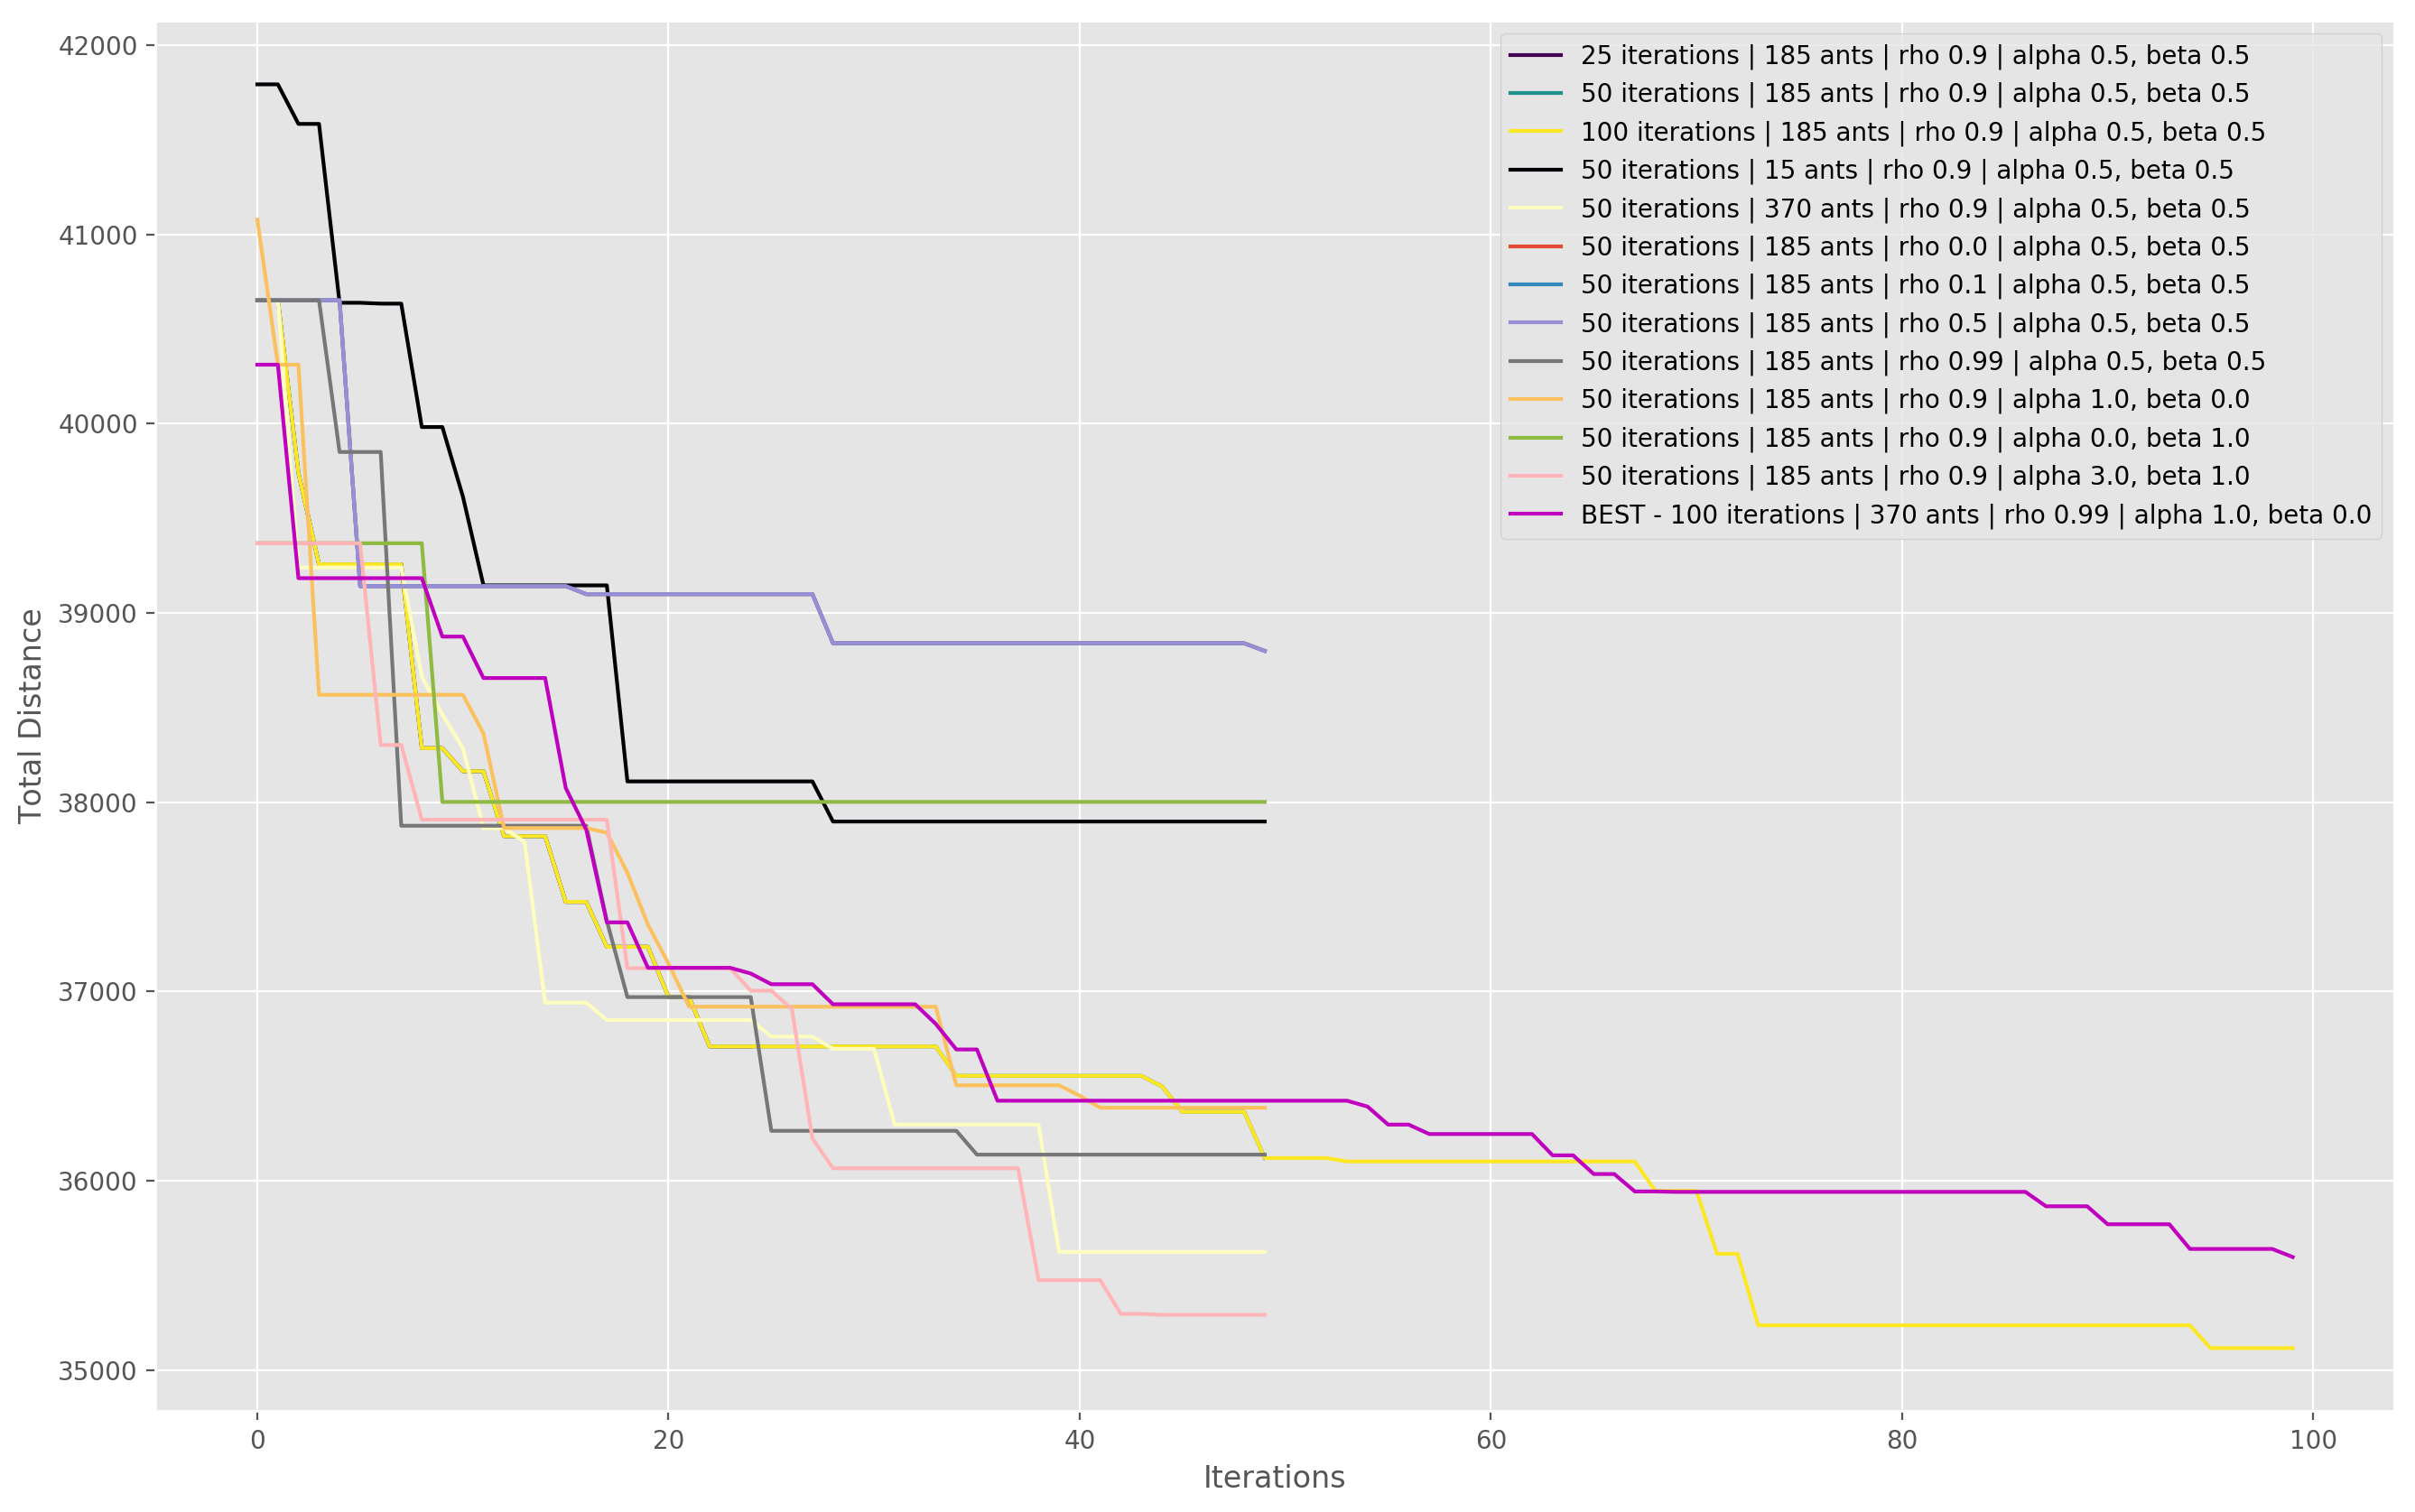
\includegraphics[width=11cm,keepaspectratio]{images/SJC2_best.png}
  \caption{Melhores soluções encontradas para a base SJC2 ao longo das repetições para todas as variações de parâmetros apresentadas até agora.}
  \label{fig:sjc2_best}
\end{figure}

\subsubsection{SJC3b}
A base de dados SJC3b é composta de 300 pontos, todos com capacidade 740, mas com demanda variável. Ela busca por 30 pontos de mediana. A análise da otimização das funções com relação ao número de iterações pode ser vista na Figura \ref{fig:sjc3b_iterations}. Assim como acontece com a base SJC1 quando usados os valores padrões para os parâmetros e 10 formigas, após a iteração 65, e até a iteração final, tanto a média quanto o desvio padrão sofrem um mudança brusca. Isso aconteceu pois em uma das execuções, após essa iteração, a distância total cai de 45726 para 2190. 

\begin{figure}[h]	
  \centering
  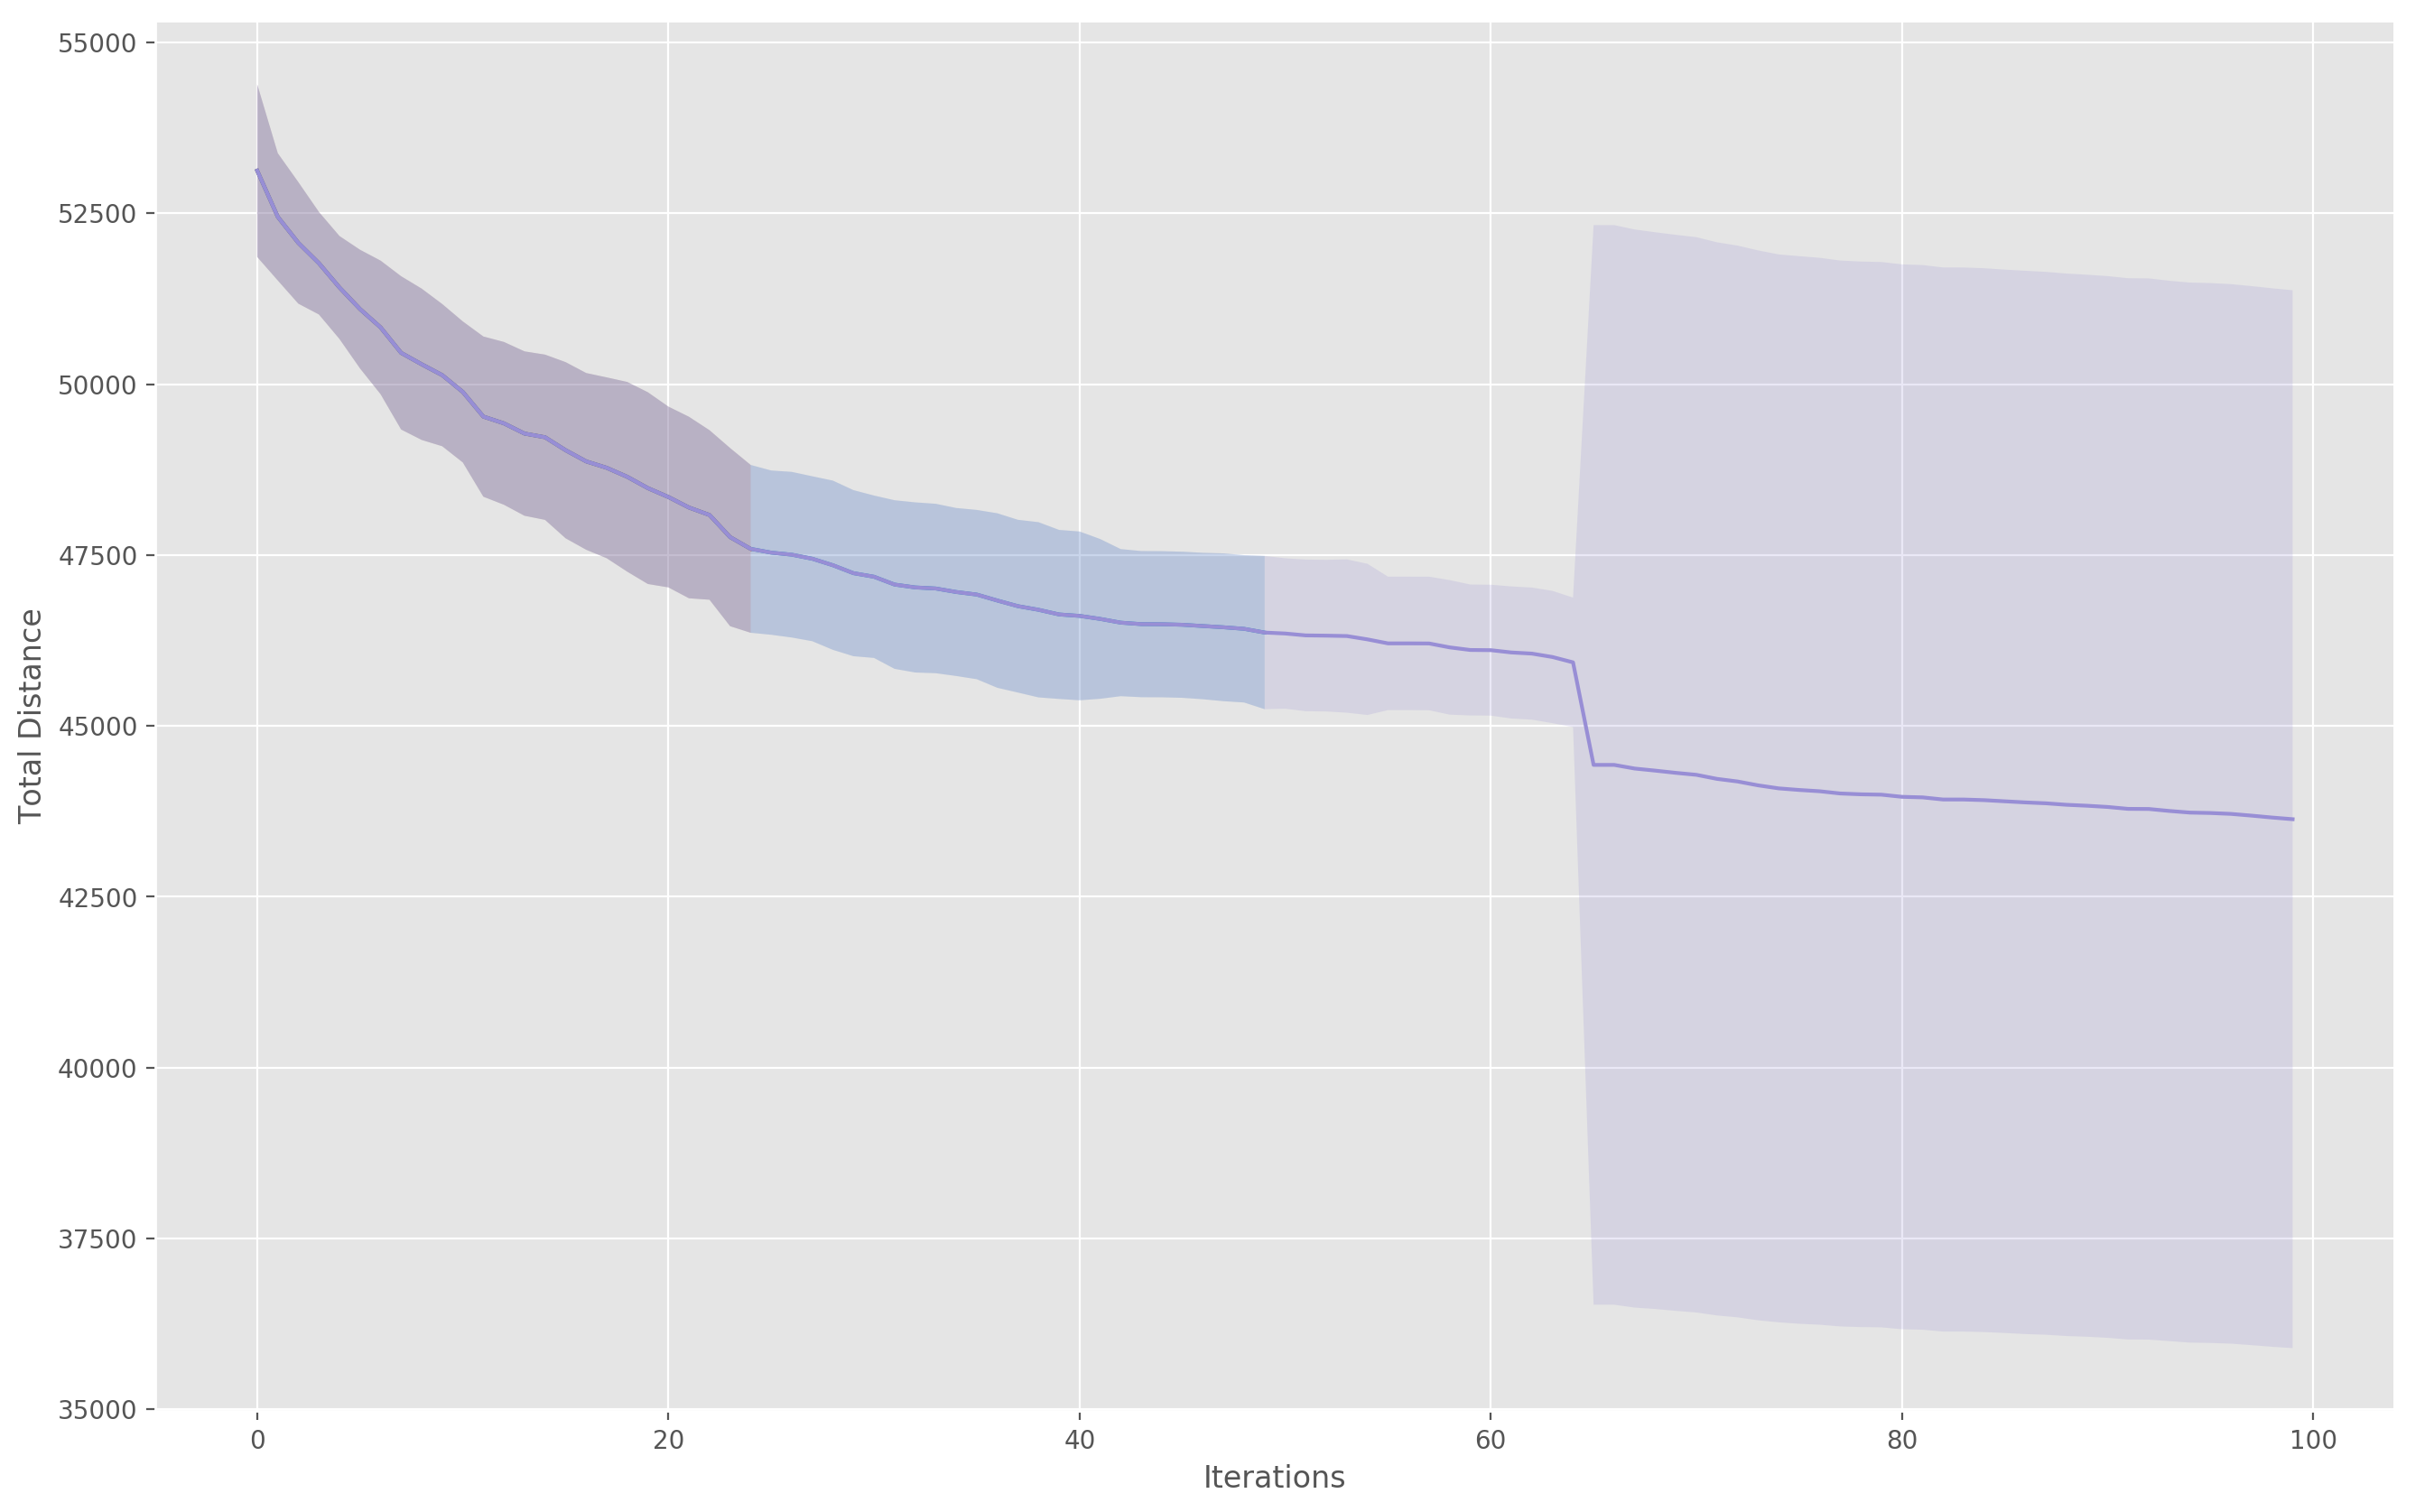
\includegraphics[width=11cm,keepaspectratio]{images/SJC3b_iterations.png}
  \caption{Média e desvio padrão para a distância da solução encontrada para base SJC3b com número de iterações variável.}
  \label{fig:sjc3b_iterations}
\end{figure}

Neste momento o leitor pode se perguntar o porque não apresentamos resultados para um número de iterações acima de 100. Não o fizemos pois, com um número 5 vezes maior de iterações, acaba que ocorre erro em todas as repetições, portanto a média do melhor global termina em 2190, como podemos ver na Figura \ref{fig:sjc3b_fail}. Esses gráficos não nos ajudam na análise, e portanto foram descartados.

\begin{figure}[h]	
  \centering
  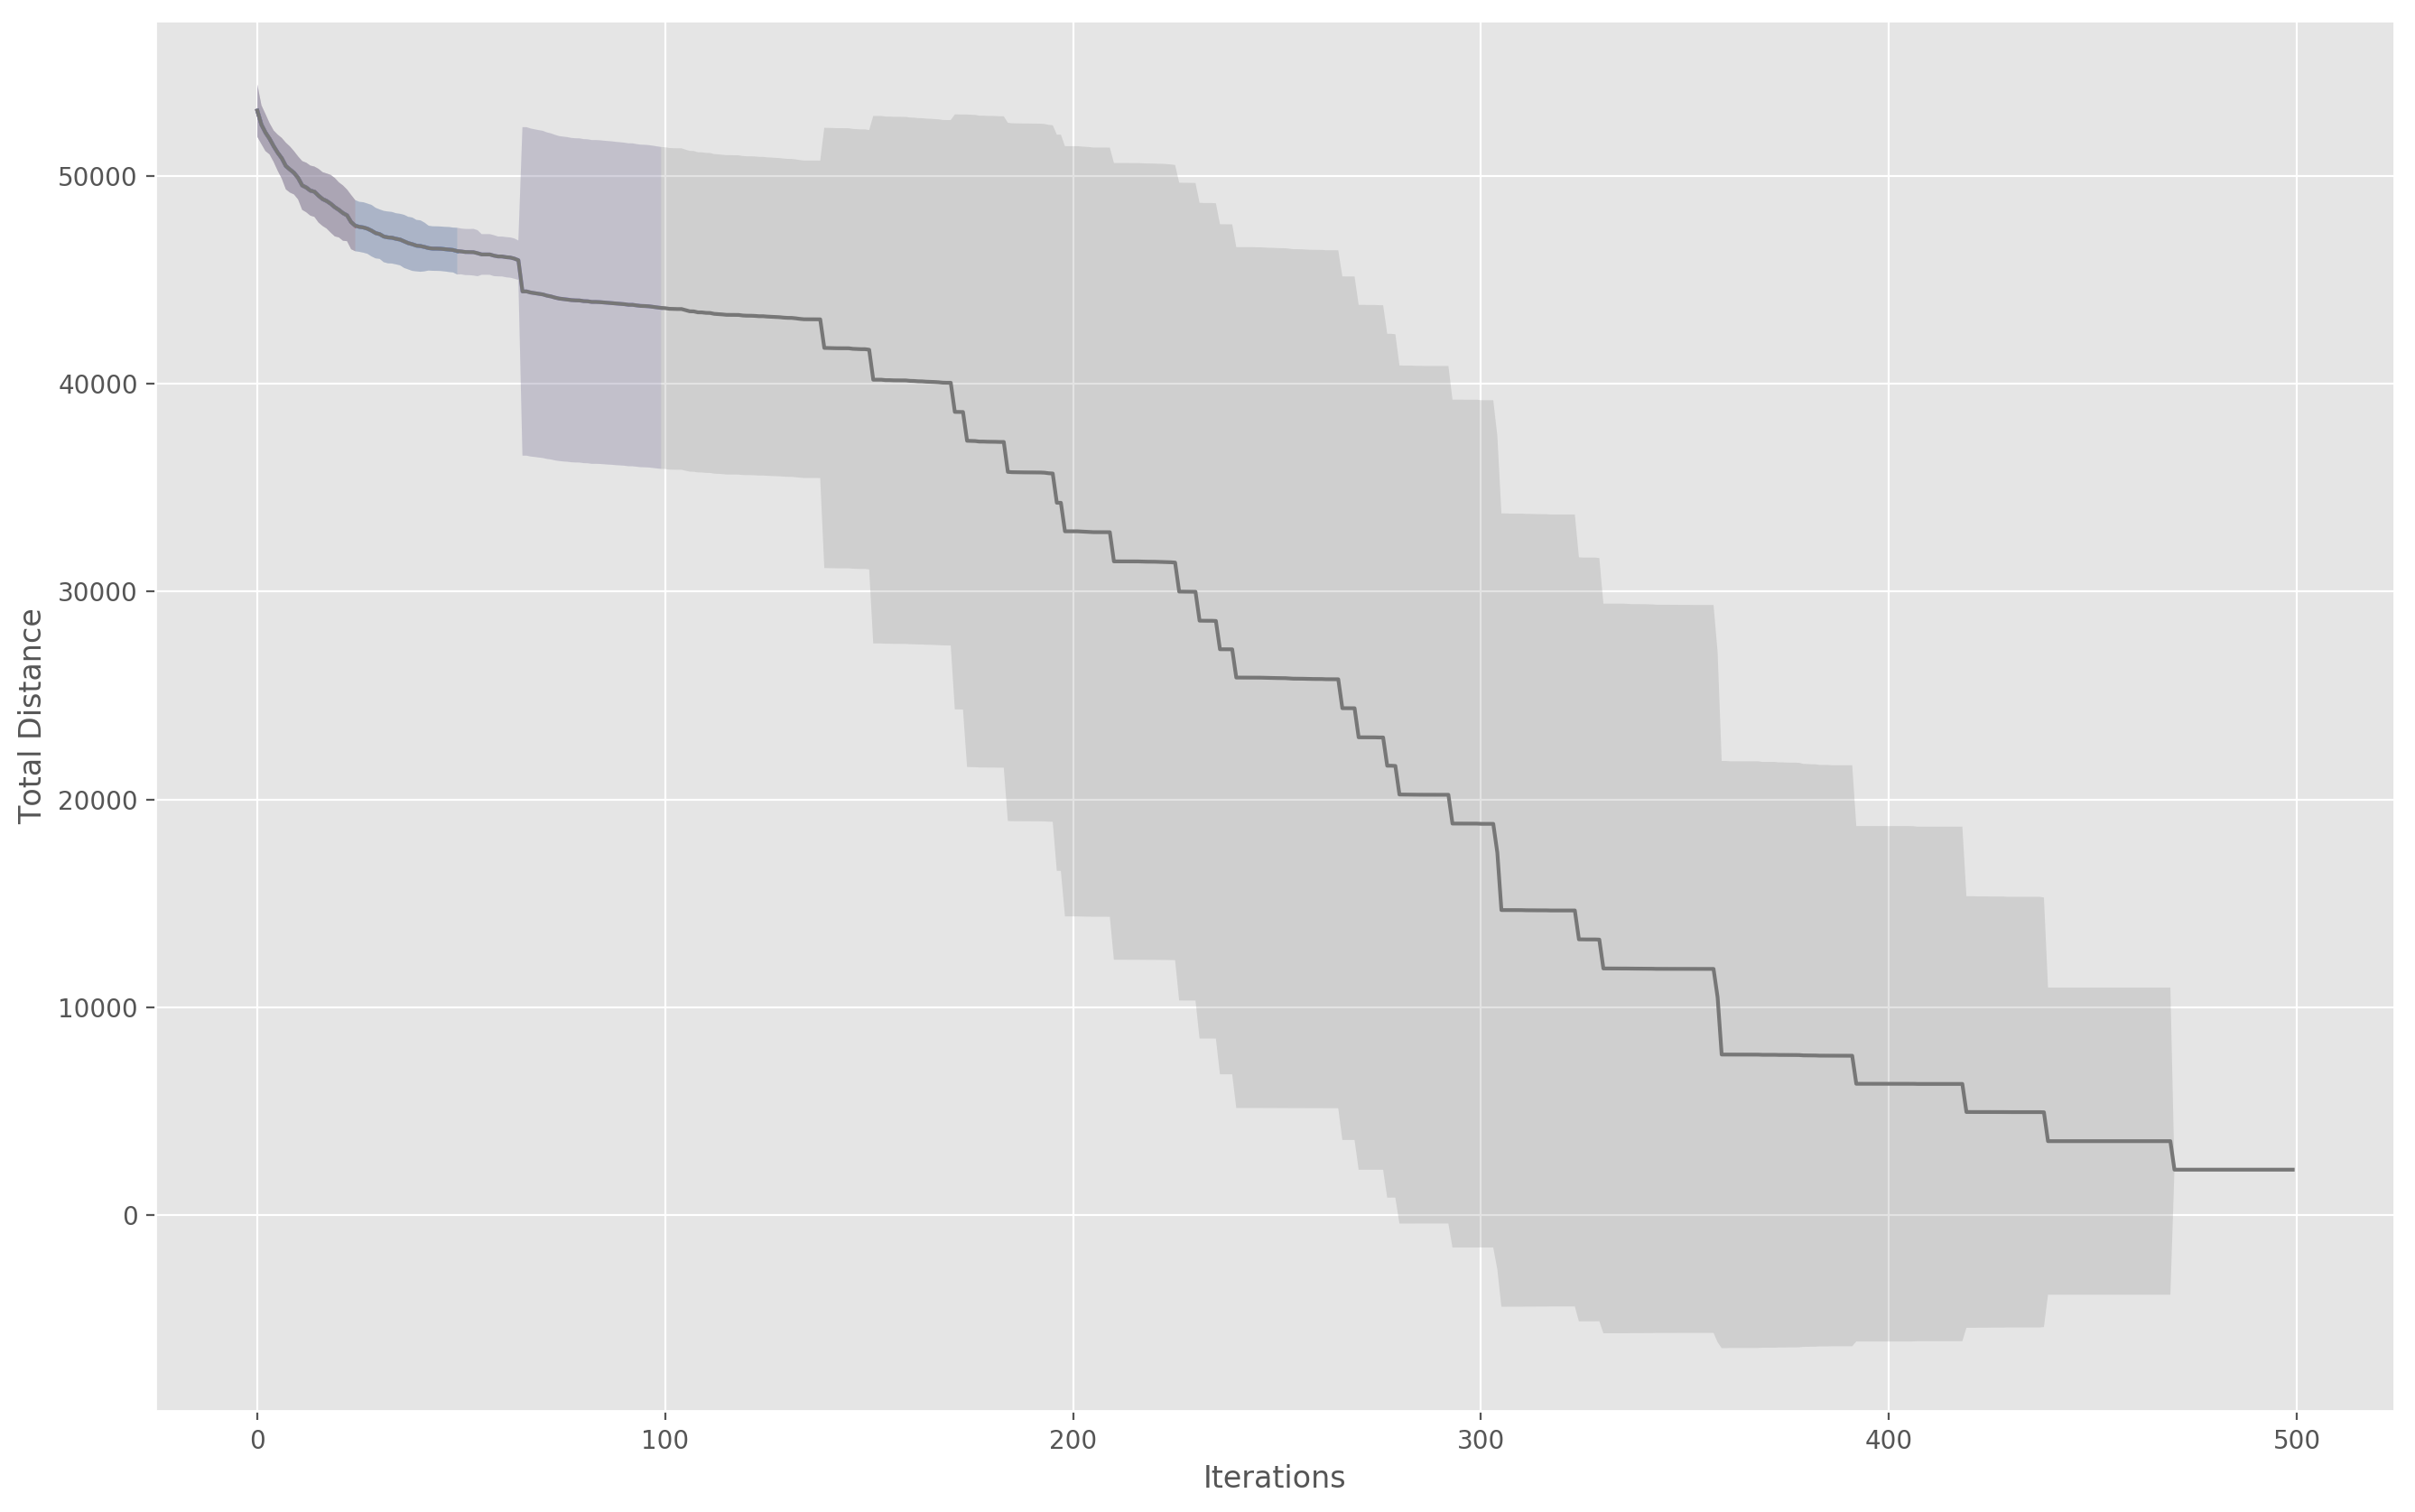
\includegraphics[width=11cm,keepaspectratio]{images/SJC3b_iterations_fail.png}
  \caption{Média e desvio padrão para a distância da solução encontrada para base SJC3b com número de formigas variável.}
  \label{fig:sjc3b_fail}
\end{figure}

No gráfico da Figura \ref{fig:sjc3b_ants} vemos que o erro ocorre novamente. No entanto, mesmo antes disso o valor médio da melhor solução global já era superior a todos os outros, fazendo com que, mais uma vez $2 * (n - p)$ formigas seja o ideal.

\begin{figure}[h]	
  \centering
  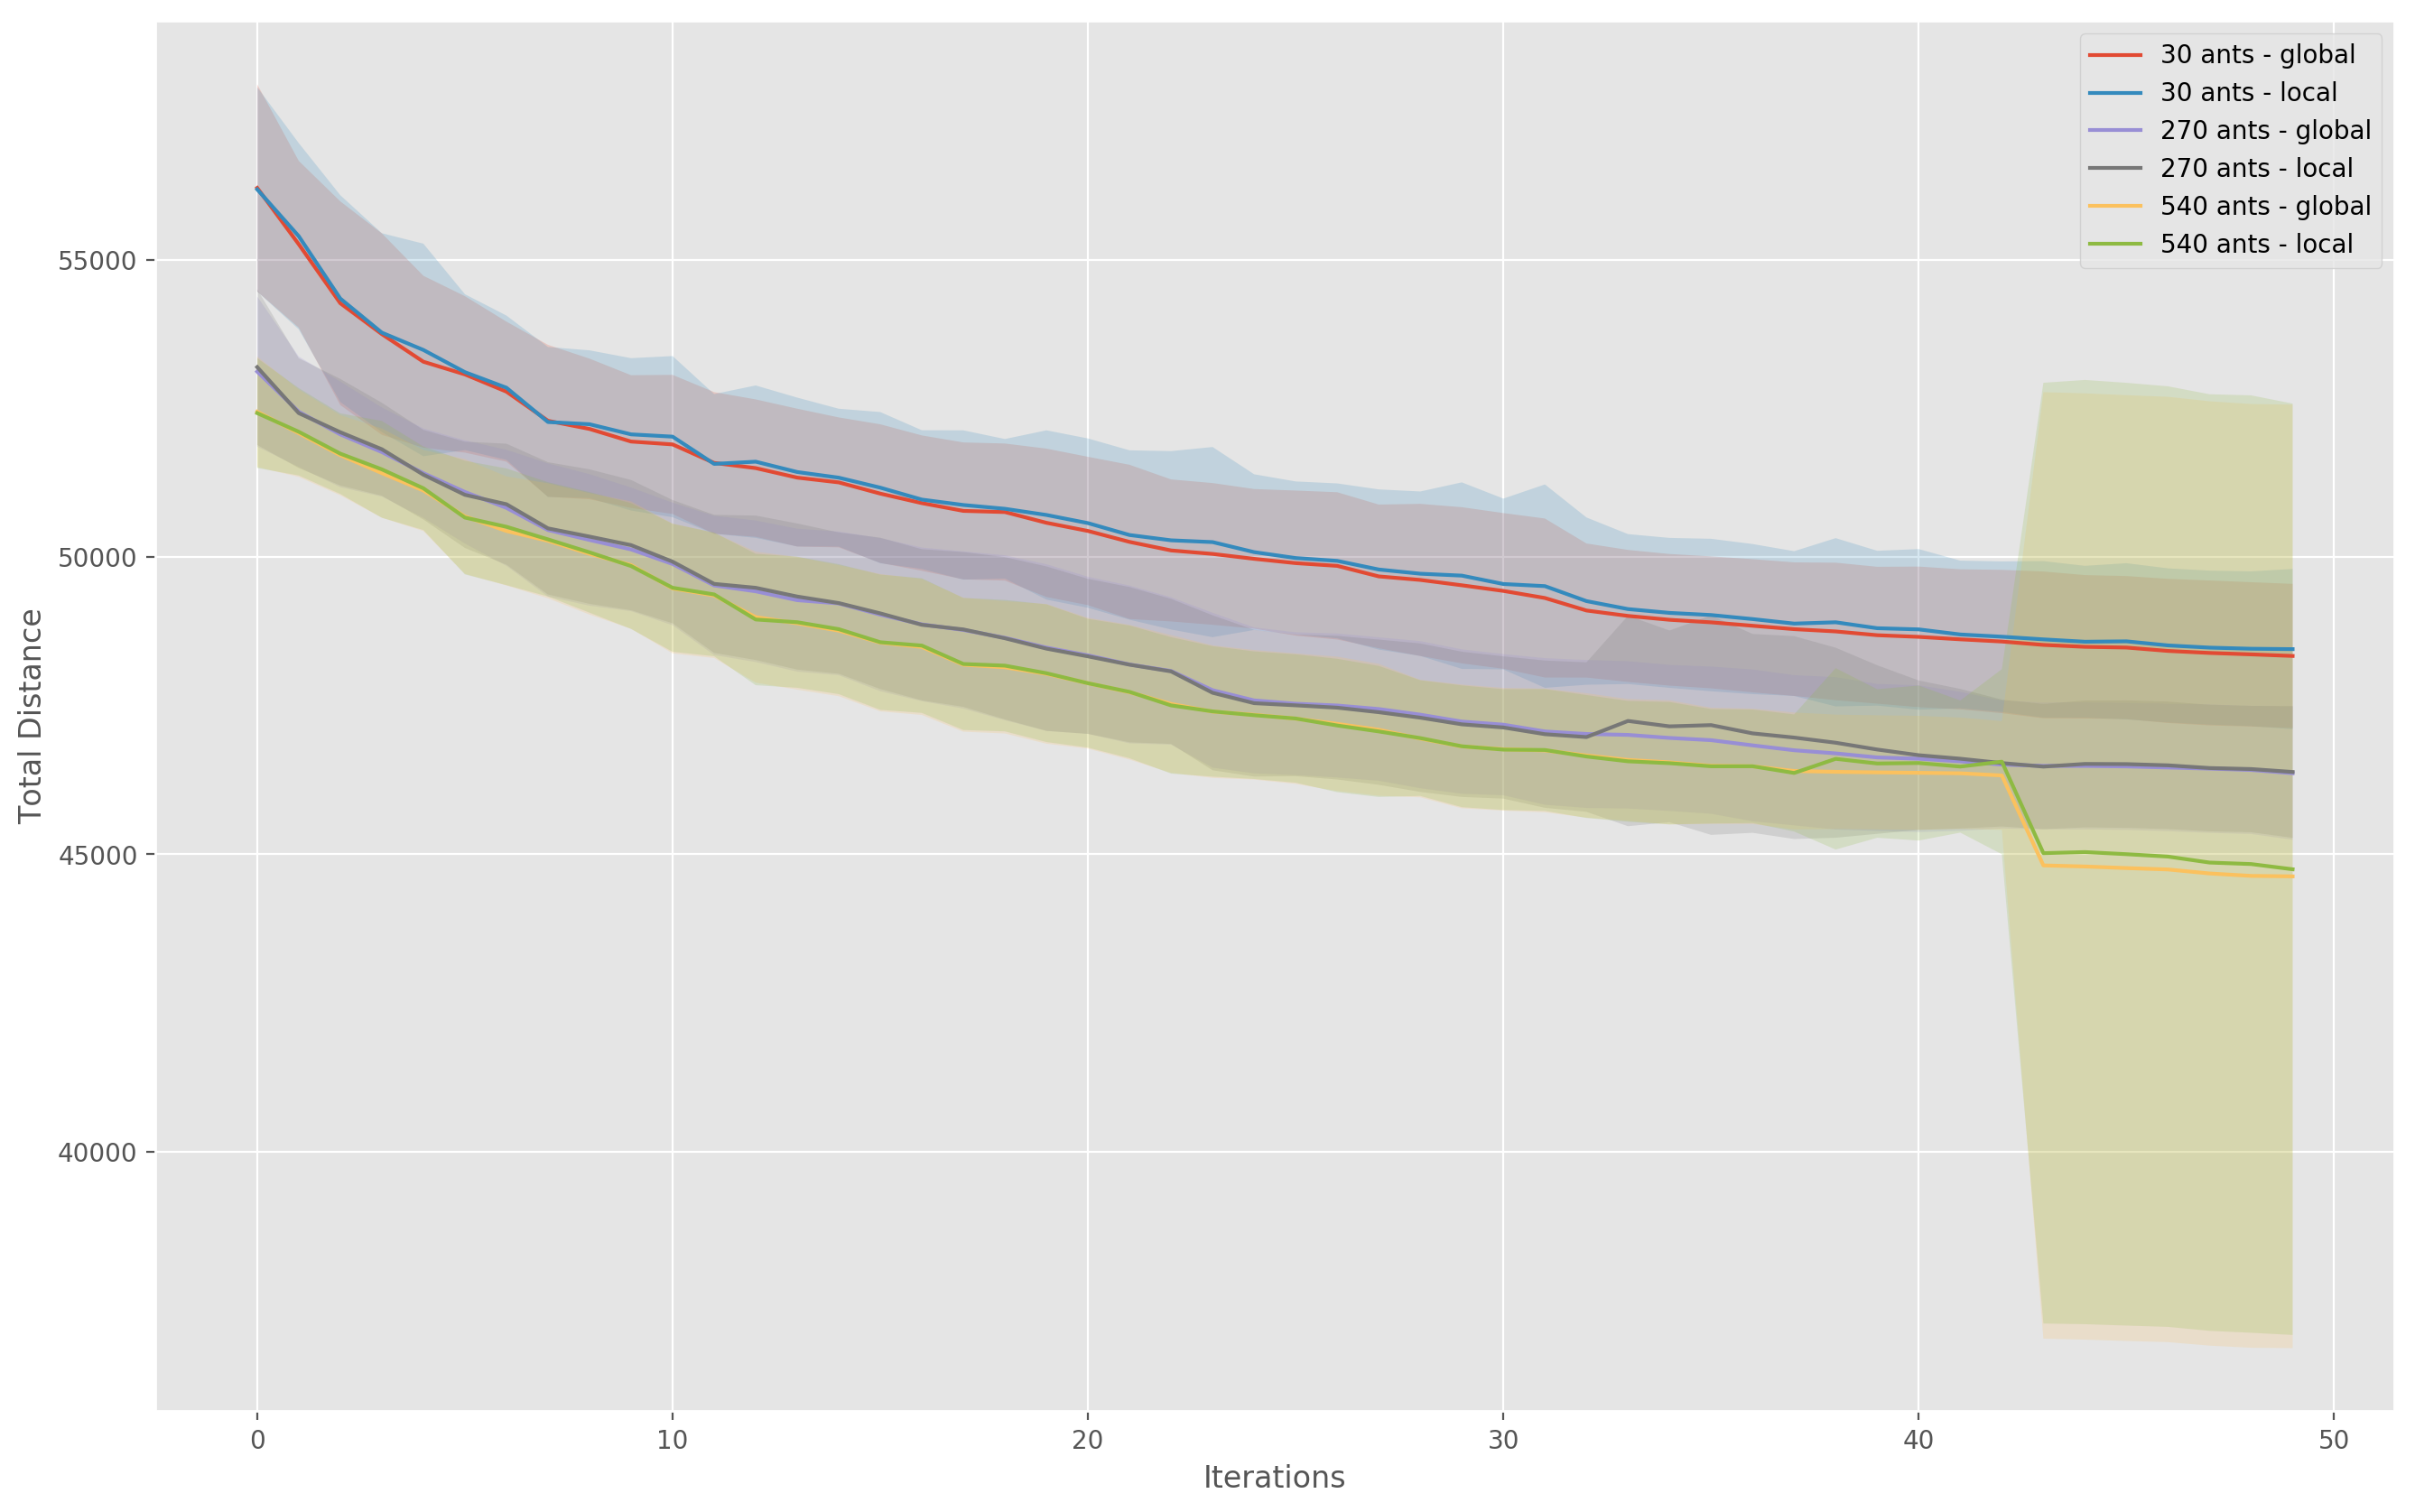
\includegraphics[width=11cm,keepaspectratio]{images/SJC3b_ants.png}
  \caption{Média e desvio padrão para a distância da solução encontrada para base SJC3b com número de formigas variável.}
  \label{fig:sjc3b_ants}
\end{figure}

Para variação da taxa de evaporação temos um cenário(Figura \ref{fig:sjc3b_rho}) semelhante às outras duas bases, porém dessa vez $\rho = 0.9$ se sobressaiu dos demais.

\begin{figure}[h]	
  \centering
  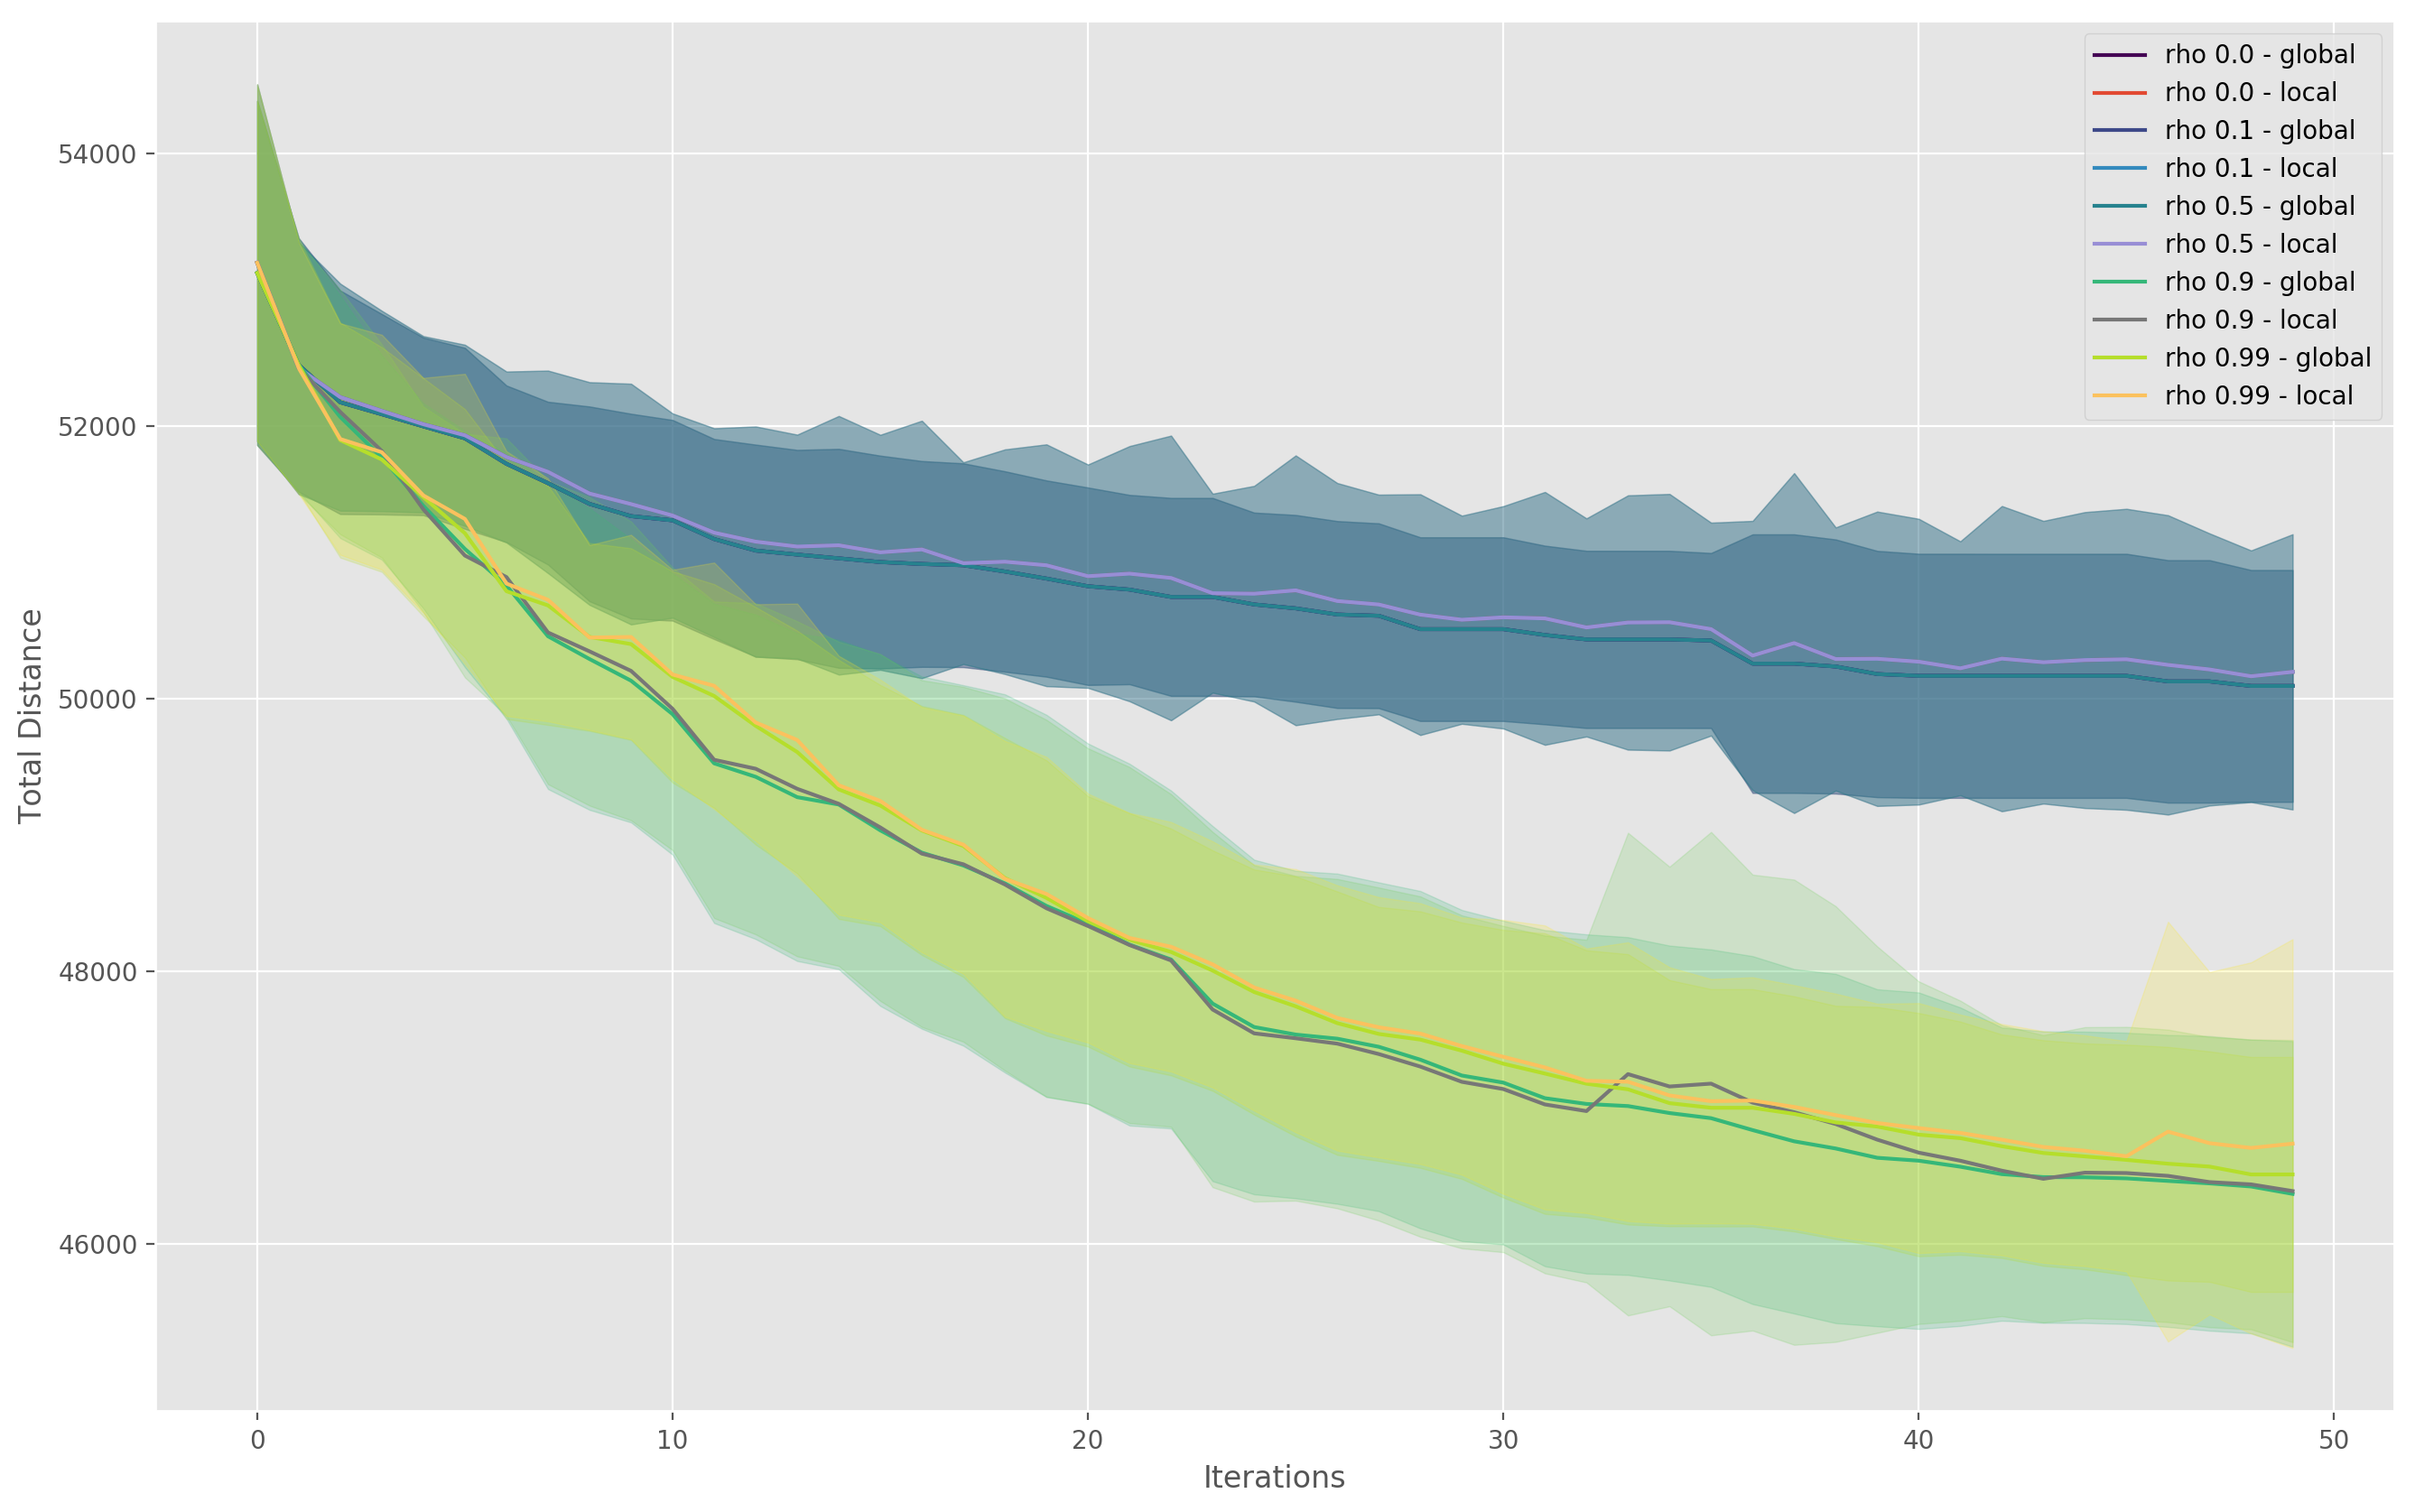
\includegraphics[width=11cm,keepaspectratio]{images/SJC3b_rho.png}
  \caption{Média e desvio padrão para a distância da solução encontrada para base SJC3b com taxa de evaporação de feromônio variável.}
  \label{fig:sjc3b_rho}
\end{figure}

Na análise dos termos $\alpha$ e $\beta$, é fácil perceber pela Figura \ref{fig:sjc3b_alpha_beta} que os parâmetros ótimos são $\alpha = 3$ e $\beta = 1$, reforçando os achados de \cite{de2005max}.

\begin{figure}[h]	
  \centering
  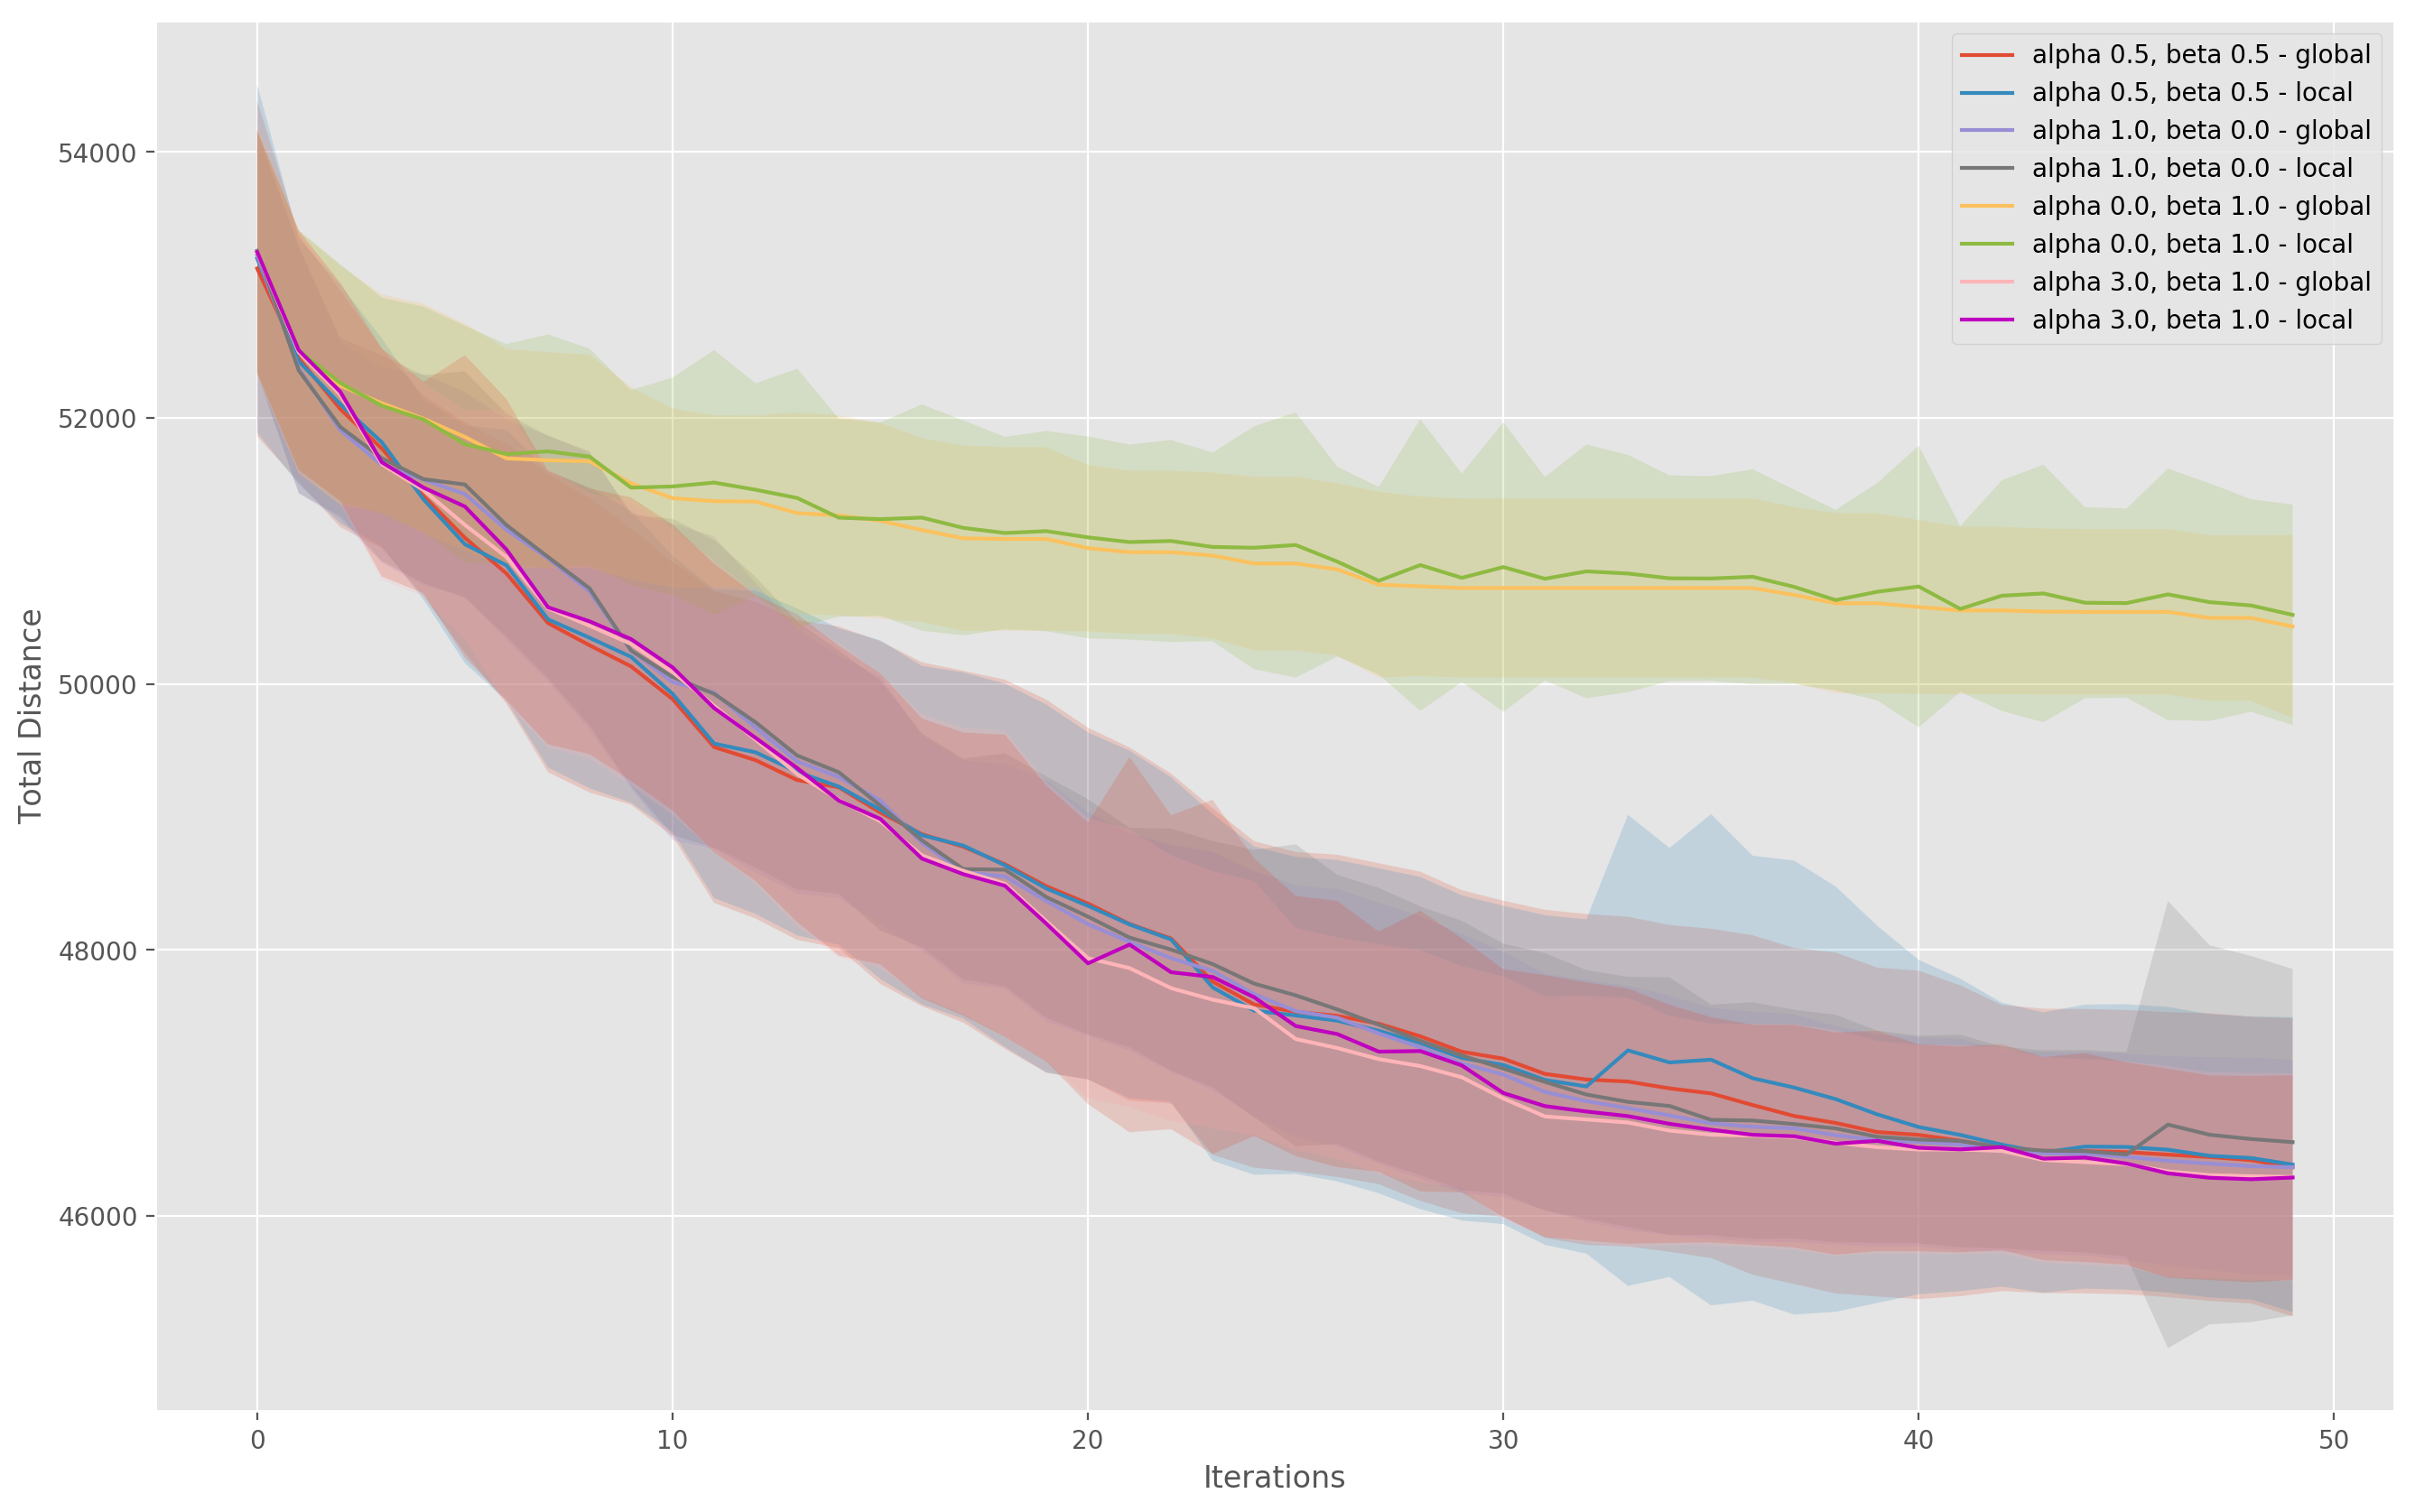
\includegraphics[width=11cm,keepaspectratio]{images/SJC3b_alpha_beta.png}
  \caption{Média e desvio padrão para a distância da solução encontrada para base SJC3b com a variação dos pesos dos feromônios e da heurística de informação no cálculo da probabilidade de escolha do nó.}
  \label{fig:sjc3b_alpha_beta}
\end{figure}

Os melhores parâmetros para a base SJC3b foram, portanto, 100 iterações, 540 formigas, $\rho = 0.9$, $\alpha=3$ e $\beta=1$. A Figura \ref{fig:sjc3b_best} mostra os melhores resultados alcançados para cada configuração. Ignorando os dois resultados bugados, vemos que a melhor solução de todas, de valor \textbf{43786.659}, foi encontrada com o conjunto dos melhores parâmetros.

\begin{figure}[h]	
  \centering
  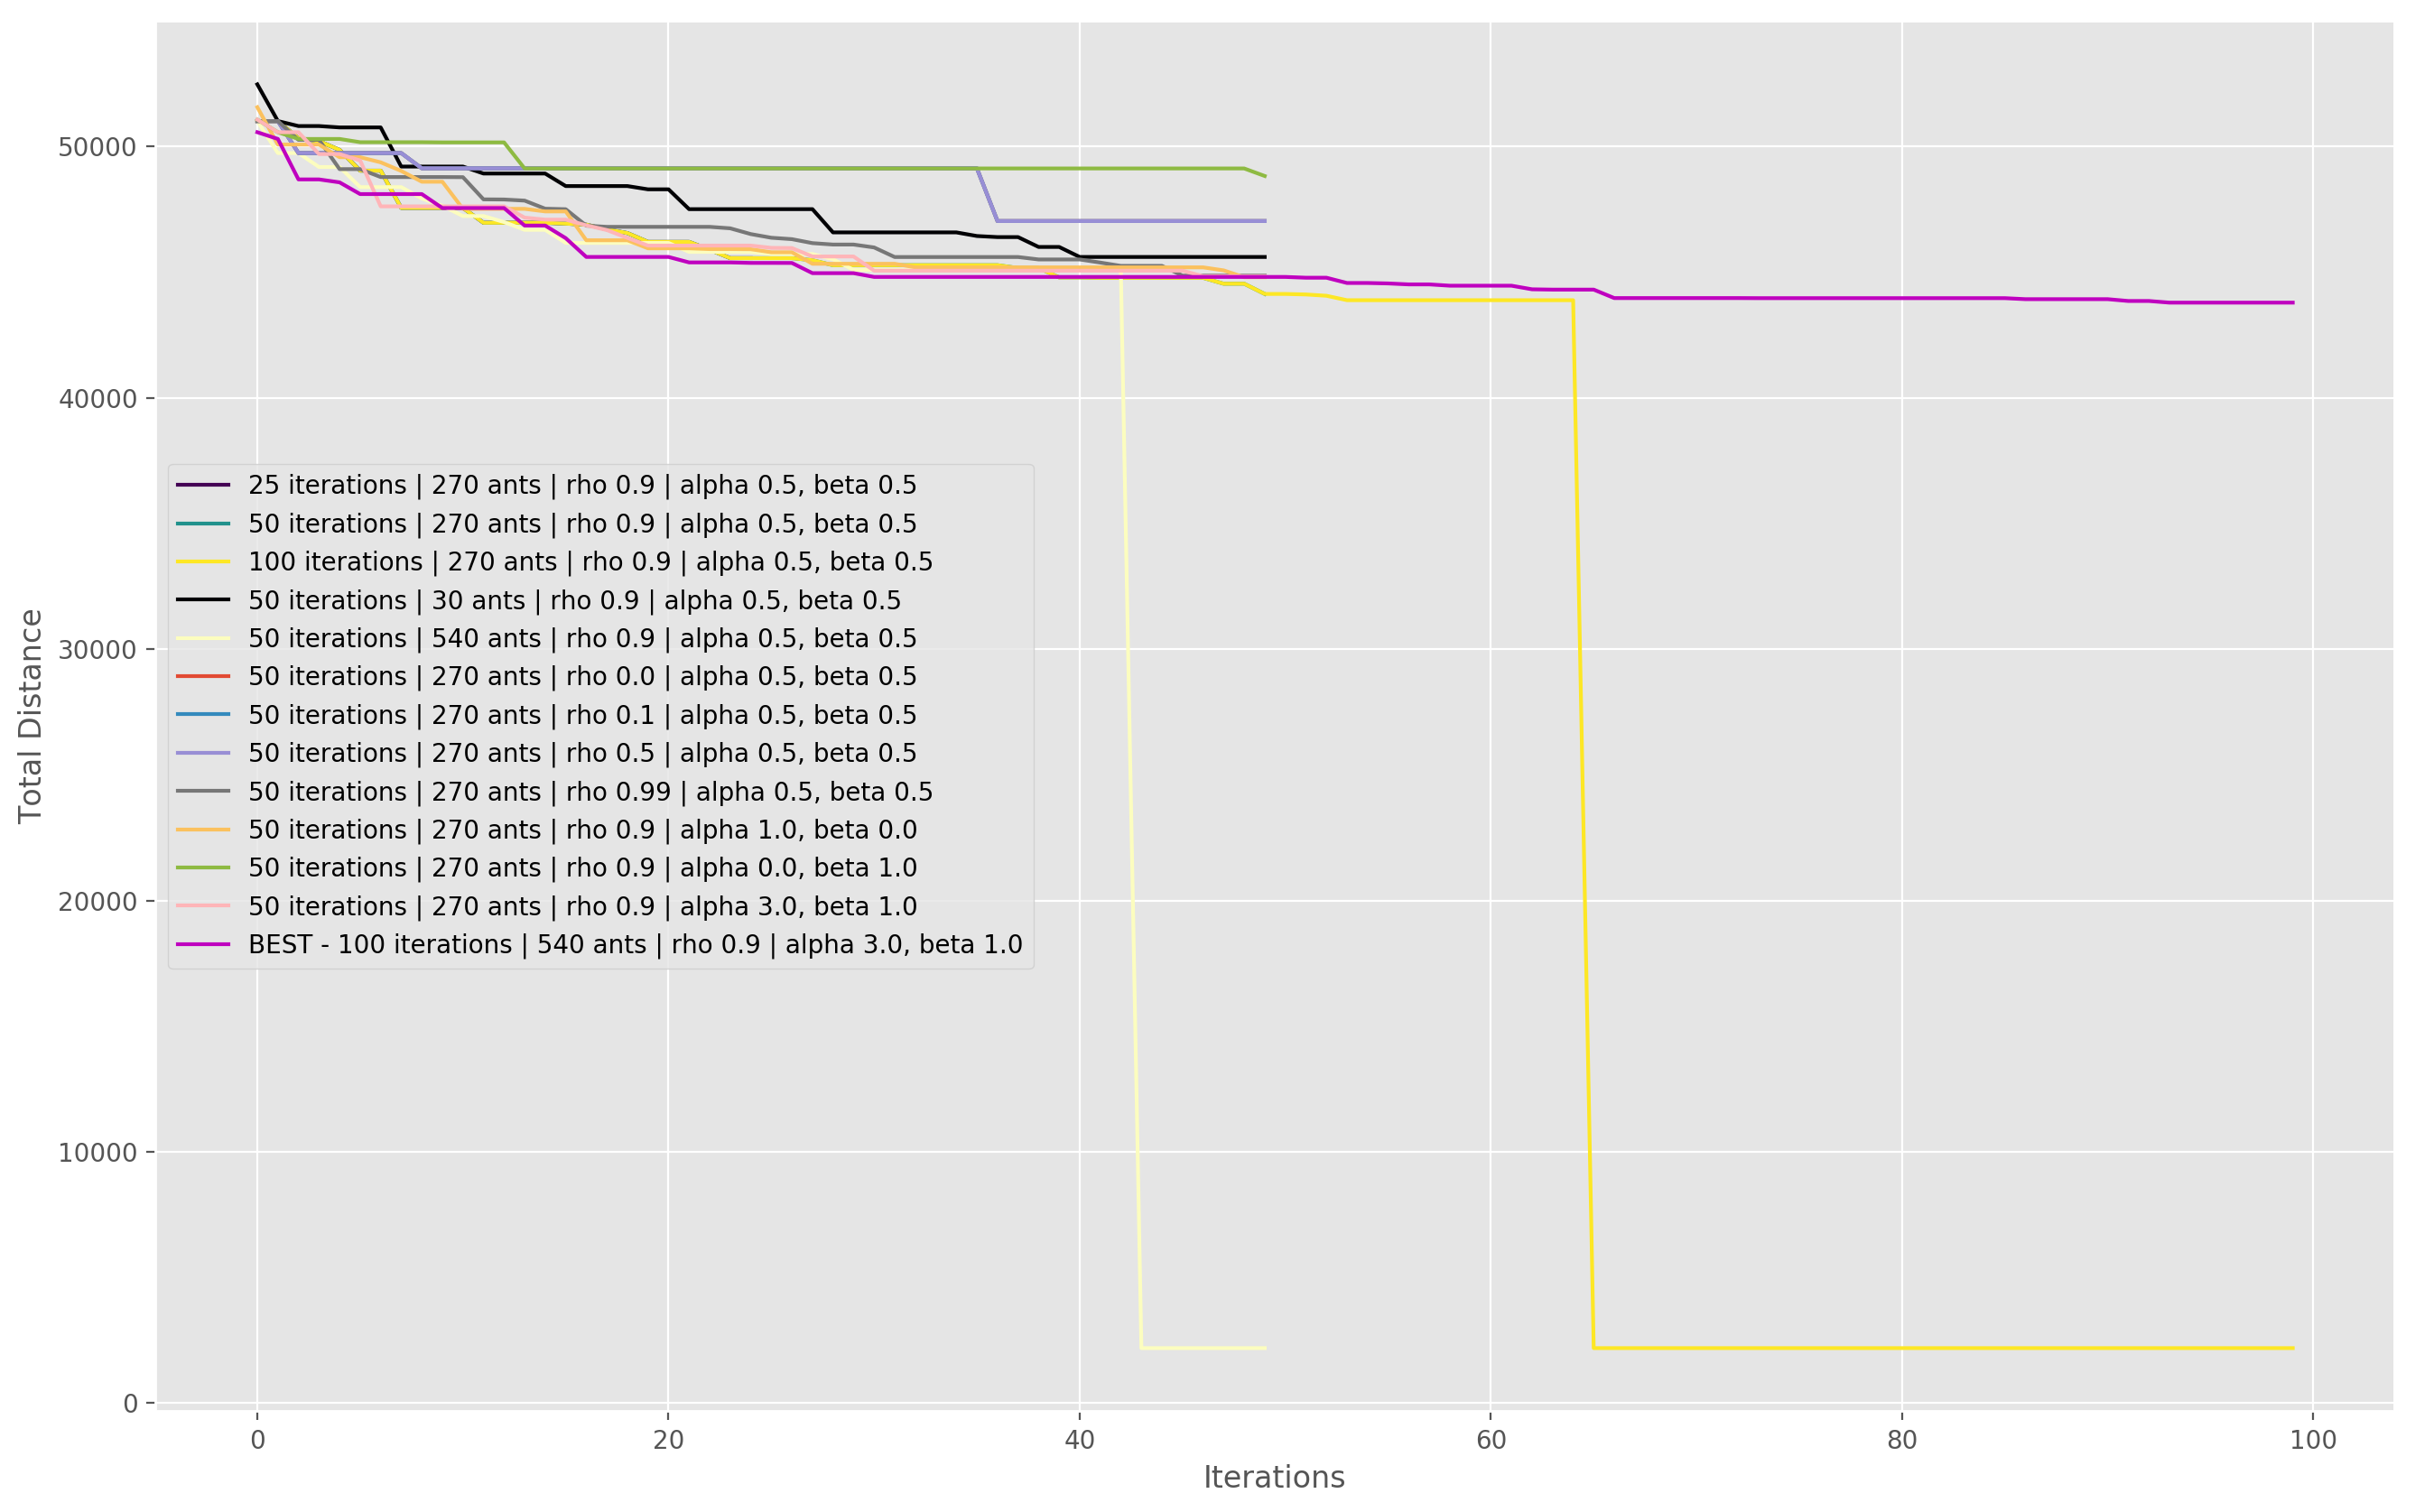
\includegraphics[width=11cm,keepaspectratio]{images/SJC3b_best.png}
  \caption{Melhores soluções encontradas para a base SJC3b ao longo das repetições para todas as variações de parâmetros apresentadas até agora.}
  \label{fig:sjc3b_best}
\end{figure}